\title{CS3210 Parallel Computing\\Assignment 1 (Part 2) Report\\[3ex]\textbf{Discrete Particle Simulation with CUDA}}
\author{Keven Loo Yuquan (A0183383Y) \& Lee Yong Jie, Richard (A0170235N)}
\date{}

\documentclass[12pt]{article}

% Margins
\usepackage[margin=2cm]{geometry}
% Math and symbols
\usepackage{amsmath}
\usepackage{amssymb}
% Syntax highlighting
\usepackage{minted}
% Inclusion of pictures
\usepackage{graphicx}
\graphicspath{{./reportAssets/}{./processedGpuResults/}}
% Better looking underlines
\usepackage{soul}
\setuldepth{Parallel}
% Combine texttt & textbf
\usepackage{bold-extra}
% No paragraph indentations
\setlength{\parindent}{0pt}
% Merge rows of table
\usepackage{multirow}
% Fixed tables
\usepackage{tabularx}
% LaTeX is dumb at deciding where figures should go
\usepackage{float}
% Enable support for coloured text blocks
\usepackage[dvipsnames]{xcolor}
% Enable URLs
\usepackage{hyperref}
% Enable references on the TOC
\usepackage[nottoc,numbib]{tocbibind}

% \bf formats a chunk of text to both texttt and textbf
\newcommand{\bt}[1]{\texttt{\textbf{#1}}}
% Center-aligned column
\newcolumntype{C}{>{\centering\arraybackslash}X}

\begin{document}
\maketitle
\setcounter{tocdepth}{1}
\tableofcontents

\pagebreak
\large{}
\section{CUDA Program Design}

The discrete particle simulation is implemented fully in CUDA, with no use of external libraries (e.g. Thrust). The overall architecture of the simulator is summarised in Figure \ref{fig:simulator-design} below.\\

\begin{figure}[H]
    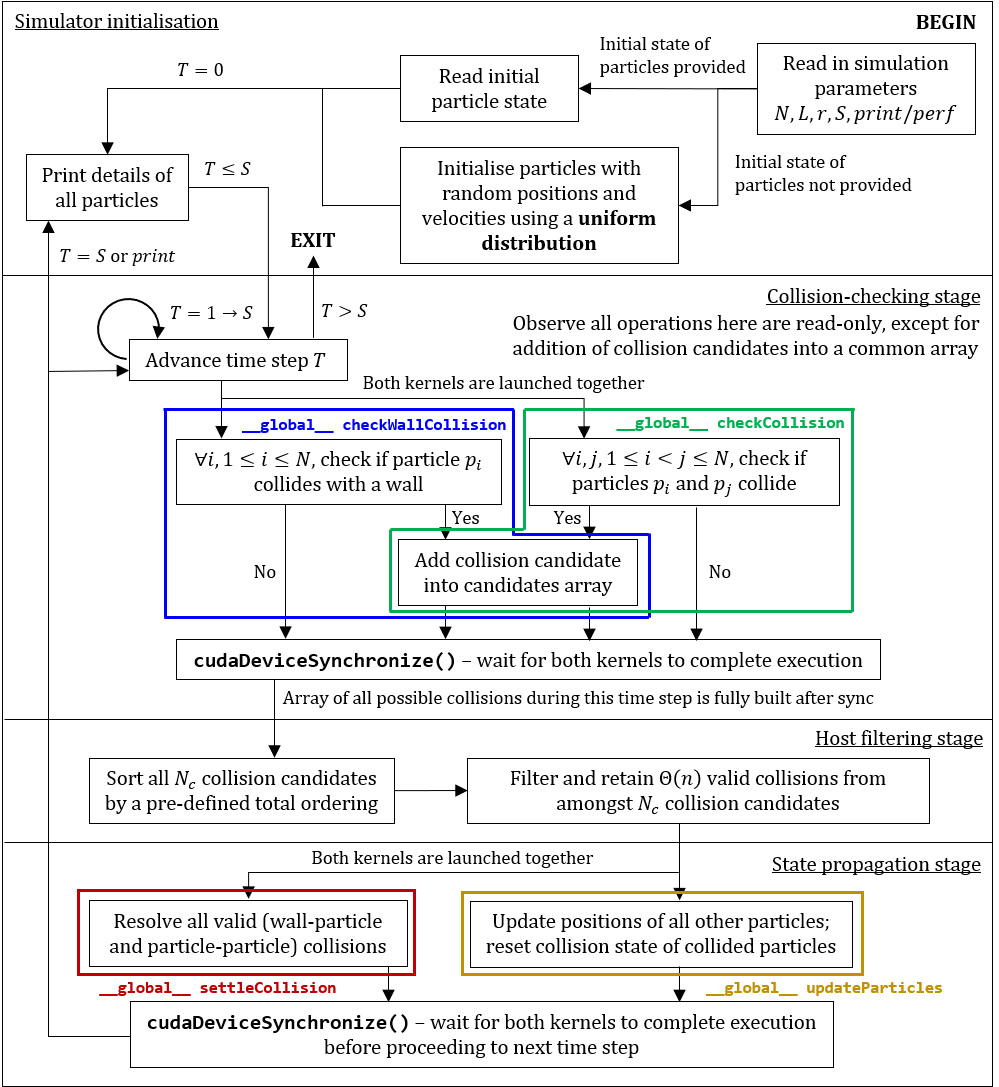
\includegraphics{chap1Flowchart-CUDA}
    \centering
    \caption{Overall simulator design for CUDA implementation}
    \label{fig:simulator-design}
\end{figure}

\pagebreak

\section{Implementation Assumptions and Details}

\subsection{Assumptions}

The first assumption from the earlier report has been removed due to changes in the testing conditions.

\begin{enumerate}
	\item A particle is involved in no more than one collision per time step.
	\begin{itemize}
		\item Implications
		\begin{enumerate}
			\item If a particle collides with a wall after any collision, it is placed at the wall at the end of that time step, and will immediately collide with the wall at the beginning of the next time step
			\item If particle $P$ collides with a particle $Q$ after any collision, it will phase through the particle $Q$ for the remainder of this time step, or will ignore $Q$ the next time step if they happen to overlap
		\end{enumerate}
	\end{itemize}
	\item All collisions between particles and with the wall are elastic (kinetic energy and momentum are conserved). 
	\item It is possible to fit all $N$ particles of radius $r$ into the square of length $L$ without overlapping.
	\begin{itemize}
		\item Implication
		\begin{enumerate}
			\item The simulation exits if one of these two conditions fail: $L < 2r$ (not possible to fit a single particle) or $Nr^2 > L^2$ (not possible to pack $N$ particles in a \ul{grid arrangement} in a square with area $L^2$)
		\end{enumerate}
	\end{itemize}
	\item The set of possible collisions $C$ satisfies a \textbf{total ordering}.
	\begin{itemize}
		\item Implication
		\begin{enumerate}
			\item For each time step $T$, it is possible to sort all collision candidates by this total ordering to determine which collisions should be prioritised over others.
		\end{enumerate}
	\end{itemize}
\end{enumerate}

\pagebreak

\subsection{Implementation Details}

Changes in general implementation details from the previous report are in \textcolor{blue}{blue}.

\begin{enumerate}
	\item If the initial state of particles are not provided, particles are generated with initial random positions and velocities using a \textbf{uniform distribution}.
	\begin{enumerate}
		\item We use the pseudo-random number generator function \texttt{rand} in the C library seeded with the number 3210.
		\item Particles are placed randomly in the square without overlapping.
	\end{enumerate}
	\item Each particle keeps track of its own state: $\textrm{ID}, x, y, v_x, v_y, \textcolor{blue}{w_c, p_c}$.
	\item Our simulation has an additional parameter \texttt{SLOW\_FACTOR} in \texttt{simulator.cu} that increases the granularity of the simulation for greater accuracy. \label{slow-factor-ref}
	\begin{enumerate}
		\item Setting \texttt{SLOW\_FACTOR} to an integer $>1$ slows the initial velocities of all particles by that factor. \texttt{SLOW\_FACTOR} should be set to a power of two to avoid introducing additional floating-point errors when dividing the particles’ velocities.
		\item The number of steps of the simulation is multiplied by \texttt{SLOW\_FACTOR} to compensate, i.e. each original step now corresponds to \texttt{SLOW\_FACTOR} ``micro-steps".
	\end{enumerate}
	\item Collisions are of two types: particle-wall collisions or particle-particle collisions. We describe a particle-wall collision as ($P$, \texttt{null}) and a particle-particle collision as ($P$, $Q$).
	\begin{enumerate}
		\item As particle-particle collisions are symmetric (i.e. $P$ collides with $Q$ $\iff$ $Q$ collides with $P$), we generate these collisions such that $P$ is the particle with lower integer ID \textcolor{blue}{to avoid duplicates}.
	\end{enumerate}
	\item When sorting collision candidates with the C library function \texttt{qsort}, we enforce this total ordering in the function \texttt{cmpCollision}. For two collision candidates  $C_1$ and $C_2$,
	\begin{itemize}
		\item[$\blacksquare$] $C_1 < C_2$ if $C_1$ occurs before $C_2$ \textcolor{blue}{(priority by time)}
		\item[$\blacksquare$] If $C_1$ and $C_2$ occur at the same time
		\begin{itemize}
			\item[$\square$] $C_1 < C_2$ if ID of $P$ in $C_1$ $<$ ID of $P$ in $C_2$ \textcolor{blue}{(priority by ID)}
			\item[$\square$] If $C_1$ and $C_2$ both involve the same particle $P$
				\begin{itemize}
					\item[$\blacksquare$] $C_1 < C_2$ if $C_1$ is a wall collision \textcolor{blue}{(priority by type)}
					\item[$\blacksquare$] If $C_1$ and $C_2$ are both particle-particle collisions
						\begin{itemize}
							\item[$\square$] $C_1 < C_2$ if ID of $Q$ in $C_1$ $<$ ID of $Q$ in $C_2$ \textcolor{blue}{(priority by ID)}
						\end{itemize}
				\end{itemize}
		\end{itemize}
	\end{itemize}
	\item For each particle in each time step, we check once if the particle collides with any of the four walls.
	    \begin{enumerate}
	        \item \textcolor{blue}{A particle is treated to have collided with a wall if it would come within a distance of $\epsilon = $ \texttt{1E-8} to the wall within that time step.}
	    \end{enumerate}
	\item All possible particle-particle collision pairs are checked for each time step. The total number of collision checks performed is thus
	\begin{align*}
	N_{potential\ collisions} 	&= N_{wall-particle} + N_{particle-particle} \\
						&= N + \frac{N(N-1)}{2} \\
						&= \Theta (N^2)
	\end{align*}
	\item Particle-wall collisions are checked by solving the trajectory equation of a particle and the position equations of the wall. The equations of the walls are $x = 0, x = L, y = 0, y = L$.
	\item \label{trajectory-calc} Particle-particle collisions are checked by solving trajectory equations of two particles during the given time step.\\
	
	Consider two particles $P$, $Q$ during a given time step $0 \leq \Delta t \leq 1$. From Pythagoras’ theorem, the distance between them is
	$$d = \sqrt{\left( \left( x_Q + v_{xQ} \Delta t \right) - \left( x_p + v_{xP} \Delta t \right) \right)^2 +
		\left( \left( y_Q + v_{yQ} \Delta t \right) - \left( y_p + v_{yP} \Delta t \right) \right)^2}$$
	or re-written in terms of deltas (differences in state)
	$$d = \sqrt{\left( \Delta x + \Delta v_x \Delta t \right)^2 +
		\left( \Delta y + \Delta v_y \Delta t \right)^2}$$
    \\
	The particles intersect when $d = 2r$, i.e. the particles touch at their circumference, hence by expanding and collecting terms we get the quadratic equation of form $A (\Delta t)^2 + B \Delta t + C = 0$,
	\begin{align*}
		\Delta x^2 + 2 \Delta x \Delta v_x \Delta t + \Delta v_x^2 (\Delta t)^2 + \Delta y^2 + 2 \Delta y \Delta v_y \Delta t + \Delta v_y^2 (\Delta t)^2 &= (2r)^2 \\
		\implies (\Delta v_x^2 + \Delta v_y^2) (\Delta t)^2 + (2 \Delta x \Delta v_x + 2 \Delta y \Delta v_y) \Delta t + (\Delta x^2 + \Delta y^2 - 4r^2) &= 0
	\end{align*}
	
	We observe that $A = (\Delta v_x^2 + \Delta v_y^2) > 0$ and thus the curve $y = d(\Delta t)$ is concave up. The discriminant for this quadratic equation, $B^2 - 4AC$, is
	$$\textrm{discriminant} = (2 \Delta x \Delta v_x + 2 \Delta y \Delta v_y)^2 - 4(\Delta v_x^2 + \Delta v_y^2)(\Delta x^2 + \Delta y^2 - 4r^2)$$
	
	If this discriminant is $\geq 0$, then the particles collide for some value of $\Delta t$, and we solve for this $\Delta t$. There are two possible roots,
	$$\Delta t = \frac{-B \pm \sqrt{\textrm{discriminant}}}{2A}$$
	
	Since the quadratic curve is concave up, we only compute and examine the first root (when the particles are approaching each other). This is
	$$\Delta t = \frac{-B - \sqrt{\textrm{discriminant}}}{2A}$$
	
	If $0 \leq \Delta t \leq 1$, then particles $P$, $Q$ collide during this time step.
	
	Note that, it is possible for $\Delta t < 0$ - this corresponds to cases where particles are overlapping from a previous step. We do not consider these as collisions in the current step and let these two particles phase through each other.
	\item \textcolor{blue}{To ensure the collision candidates array can accommodate $\Theta(N^2)$ potential collisions (in the limit of large $N$ when particle-particle collisions dominate), we dynamically allocate an array in managed memory with sufficient space to store $N^2 / 2$ collision structs.}
	\begin{itemize}
	    \item \textcolor{blue}{Unfortunately, \texttt{cudaMallocManaged()} fails to allocate the required space when $N = 64000$.}
	\end{itemize}
\end{enumerate} 

\pagebreak

\section{Problem Decomposition}

\subsection{Host-device Work Division}
The entire simulation can be divided into multiple phases:
\begin{enumerate}
    \item \textbf{[Host]} Initialisation: reading in parameters and optionally initial particle states; randomising particles otherwise
    \item \textbf{[Host + device]} Step-wise simulation: see below
    \item \textbf{[Host]} Output of simulation state: printing states of all particles ($S=0$ and $S=N$ for \texttt{perf} mode, or all steps for \texttt{print} mode)
\end{enumerate}

We decided to let the \textbf{host} perform the simulator initialisation and output of the simulation stage, since these tasks are inherently serial.
\begin{itemize}
    \item The initialisation of particle with random positions is serial as our simulator guarantees that particles are placed without overlapping, requiring each new particle placed to be checked against all previous particles placed.
    \item The printing of the simulation state can be parallelised, but this would make the order of the output indeterminate and difficult to check.
\end{itemize}

For step-wise simulation, we see from Figure \ref{fig:simulator-design} that computing a single step comprises three distinct stages, two of which contain multiple tasks:
\begin{enumerate}
    \item \textbf{[Device]} Collision-checking: particle-wall and particle-particle
    \item \textbf{[Host]} Filtering: prioritising valid collisions
    \item \textbf{[Device]} State propagation: resolving collisions and updating positions
\end{enumerate}

The three stages must be completed serially for each step, requiring inter-stage synchronisation points. However, within each stage, it is possible to complete the tasks in parallel, eliminating the need for intra-stage synchronisation points.
\begin{enumerate}
    \item Synchronisation between the host and device between each stage is achieved with a call to \texttt{cudaDeviceSynchronize()}
    \item During collision-checking, each CUDA thread is only reading the current state of its assigned particle(s)
        \begin{itemize}
            \item For a given particle $P$, this allows its collision checks with walls and other particles to proceed concurrently
            \item However, to prevent race conditions, synchronisation is required when a CUDA thread
            \begin{itemize}
                \item adds a new collision candidate to the global array, and
                \item increments the number of collision candidates in the global counter
            \end{itemize}
        \end{itemize}
    \item During state propagation, a particle's state will only be updated by one CUDA thread
        \begin{itemize}
            \item If a particle was involved in a collision, its state will be updated when the collision is resolved
            \item Otherwise, its state will be updated when its next position is computed; the collision status of collided particles will also be reset back to \texttt{false} during this single pass
        \end{itemize}
\end{enumerate}

Therefore, we decided to represent each task in each of these two stages with a separate kernel, for a total of four. They are 
\begin{enumerate}
    \item \texttt{\_\_global\_\_ checkWallCollision} - checks all particle-wall collisions
    \item \texttt{\_\_global\_\_ checkCollision} - checks all particle-particle collisions
    \item \texttt{\_\_global\_\_ settleCollision} - resolves all valid collisions after filtering
    \item \texttt{\_\_global\_\_ updateParticles} - updates state of uncollided particles; resets collision status of collided particles
\end{enumerate}

For a given time step, we launch the first two kernels together during the first stage. Similarly, after the host has completed filtering out the valid collisions, we launch the latter two kernels together during the third stage.\\

We opted to let the \textbf{host} continue to perform the sorting and filtering of the valid collisions, since
\begin{itemize}
    \item A good parallel sorting algorithm on the GPU is difficult to implement by hand, without the use of external libraries (e.g. Thrust)
    \item Filtering out valid collisions is inherently serial since selecting an earlier may invalidate later collisions, due to the constraint that a particle can only collide once in a given time step
\end{itemize}

\subsection{Memory Choices}

Our simulator makes use of the following variables that are shared between the host and device:
\begin{itemize}
    \item Simulation parameters \texttt{N}, \texttt{l}, \texttt{r} and \texttt{S}
    \item Constant parameters \texttt{minPosMargin}, \texttt{maxPosMargin} and \texttt{maxPos} that depends on the above values of \texttt{l}, \texttt{r} and the floating-point error allowance \texttt{EPS = EDGE\_TOLERANCE = 1E-8}
    \item Shared particle array \texttt{ps}
    \item Shared collision candidates array \texttt{cs}
    \item Shared particle collision status array \texttt{states}
    \item Shared counter for number of entries in the \texttt{cs}, \texttt{numCollisions}
\end{itemize}

Since the following variables are required by all CUDA threads and does not change throughout a simulation, we opted to place the following in \textbf{constant memory}.
\begin{itemize}
    \item Variables: \texttt{N}, \texttt{l}, \texttt{r}, \texttt{S}, \texttt{minPosMargin}, \texttt{maxPosMargin} and \texttt{maxPos}
    \item The constant memory is slow and read-only, but is \textbf{cached}
    \item If all threads in a warp are reading the same address from the \textit{constant cache}, it is significantly faster than the alternatives
        \item Accesses to the same address in global memory by different warps cannot be coalesced into a single memory transaction, increasing memory traffic.
        \item Accesses to the same address in shared memory by threads in a warp lead to \textbf{bank conflicts}, leading memory requests to be serialised.
\end{itemize}

We opted to avoid the use of shared memory in favour of local memory for multiple reasons:
\begin{enumerate}
    \item Local memory is faster than shared memory, and avoids the issue of \textbf{bank conflicts} that arise from multiple threads in a warp accessing an address in the same bank.
    \item For kernels \texttt{checkWallCollision} and \texttt{checkCollision}, a CUDA thread is assigned particle(s) on which to perform a computation - where possible, the assigned structs are copied entirely into local memory to reduce strain on the memory subsystem.
    \item For the kernel \texttt{settleCollision}, a CUDA thread is assigned a collision struct which we also copied entirely into local memory.
    \item For the kernels \texttt{settleCollision} and \texttt{updateParticles}, most of the work involves updating the state of the associated particles in the global memory.
    \begin{itemize}
        \item We rely on the L1 cache on each of the Streaming Multiprocessors (SMs) to reduce the read latency for particle attributes from global memory.
        \begin{itemize}
            \item Since the 64KB of fast memory on each SM is split between the L1 cache and shared memory, avoiding the use of shared memory allows us to prioritise the fast memory for the L1 cache (see Section \ref{subsection:cache-preference-optimisation})
        \end{itemize}
    \end{itemize}
    \item Reduces the length of the CUDA program by avoiding the need to manually shuffle data between local, shared and global memory.
\end{enumerate}

We opted to use \textbf{managed memory} for convenience, with its corresponding performance loss. Since the size of the arrays scale with the number of particles $N$, this allows the unified memory subsystem to manage and shuffle data between the host's RAM and the device's global memory, as required for computation.

\subsection{Kernel Design}

Notable implementation details for any of the kernels are discussed here.\\

For the kernels \texttt{checkWallCollision} and \texttt{checkCollision}, synchronisation is required to ensure correct execution when the shared counter \texttt{numCollisions} and shared collisions array \texttt{cs} are updated by multiple CUDA threads.
\begin{itemize}
    \item We use the provided atomic function \texttt{atomicAdd} to add \texttt{1} to the shared counter \texttt{numCollisions} in global memory when a CUDA thread computes a new collision candidate.
    \item Since \texttt{atomicAdd} returns the previous value at that memory address, this gives each CUDA thread a unique index in the \texttt{cs} array to add its collision candidate to.
\end{itemize}

\pagebreak

\subsection{Grid and Block Dimensions}

We used 0-based indexing for this entire section, and $flr$ denotes the floor function.\\

For the kernels \texttt{checkWallCollision} and \texttt{updateParticles}, we only need a single pass over all $N$ particles to perform computations. Therefore, we decided to launch both kernels with the following parameters:
\begin{itemize}
    \item 1D kernel grid: $flr((N + 32 - 1) / 32)$  blocks
    \item 1D thread block: 32 threads
\end{itemize}

Since the thread block is 1D with 32 threads, we assign it a contiguous 32-particle section of the particle array \texttt{ps}, with each thread responsible for performing computations on a single particle. This increases the spatial locality of memory accesses to global memory (where \texttt{ps} resides), allowing memory accesses by threads in the same warp to be coalesced to reduce memory traffic.\\

The mapping of blocks in the kernel grid $B_i$ to sections of the array is shown in Figure \ref{fig:linearParticleMapping}.

\begin{figure}[H]
    \centering
    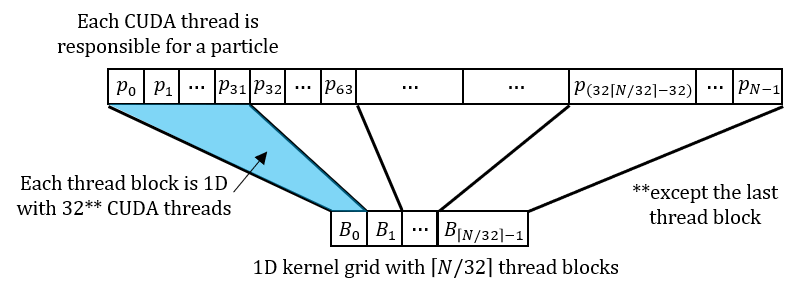
\includegraphics[width=0.9\textwidth]{reportAssets/chap3particleArrayMapping.png}
    \caption{Mapping of 1D particles array to 1D kernel grid}
    \label{fig:linearParticleMapping}
\end{figure}

For the kernel \texttt{settleCollision}, we only need a single pass over the array of $N_c$ valid collisions (note that $N_c$ varies with time step $S$). Thus, similar to the above, we launch the kernel with the following parameters:
\begin{itemize}
    \item 1D kernel grid: $flr((N_c + 32 - 1) / 32)$ blocks
    \item 1D thread block: 32 threads
\end{itemize}

The mapping of blocks in the thread grid $B_i$ to sections of the array is shown in Figure \ref{fig:linearCollisionMapping}.

\begin{figure}[H]
    \centering
    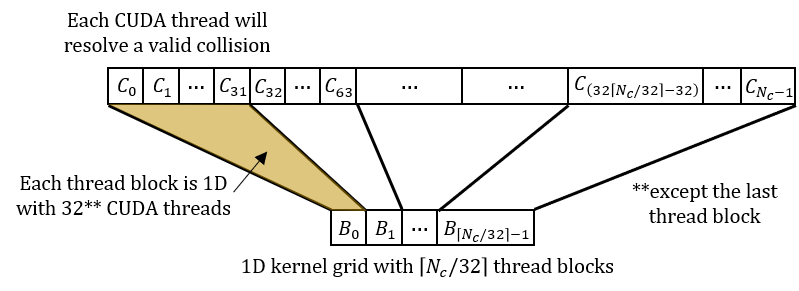
\includegraphics[width=0.9\textwidth]{reportAssets/chap3collisionArrayMapping.png}
    \caption{Mapping of 1D collisions array to 1D kernel grid}
    \label{fig:linearCollisionMapping}
\end{figure}

The mapping for the kernel \texttt{checkCollision} is not as trivial. Since we only check particle-particle collision pairs for $p_i$ and $p_j$ where $0\leq<i<j<n$ (where $i$, $j$ are the indices of the particle in the array \texttt{ps}, we can visualise all the computations to be performed for each time step in the upper diagonal of a matrix, as shown in Figure \ref{fig:collisionMatrix}.

\begin{figure}[H]
    \centering
    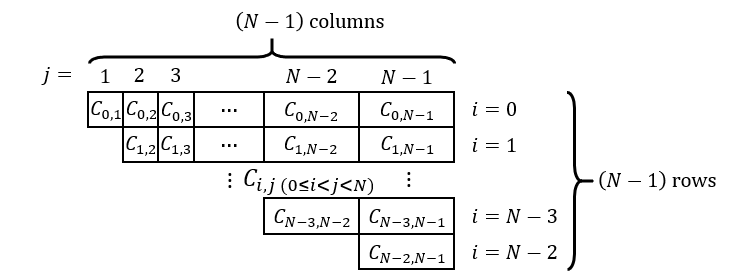
\includegraphics[width=0.9\textwidth]{reportAssets/chap3ppCollisionMatrix.png}
    \caption{Matrix of particle-particle computations}
    \label{fig:collisionMatrix}
\end{figure}

We considered distributing the $i$th row of the matrix to the $i$th thread block in a 1D kernel grid of $(N - 1)$ blocks to compute. However, this leads to an uneven distribution of work amongst blocks, since the amount of potential collisions to compute for the $i$th row is $(N - 1 - i)$. Worse still, it does not fully utilise the GPU since many warps would be executing with fewer than 32 active threads.\\

Since the upper half of the matrix resembles a triangle, we decided to "fold" the lower half of the matrix onto the upper half, by reflecting it in both axes and stitching it together to form a rectangle, as shown in Figure \ref{fig:collisionMatrixFolded}.

\begin{figure}[H]
    \centering
    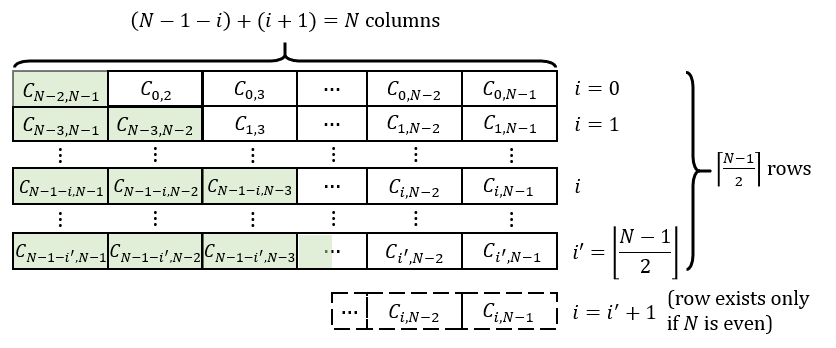
\includegraphics[width=0.9\textwidth]{reportAssets/chap3ppCollisionMatrixFolded.png}
    \caption{Folded matrix of particle-particle computations}
    \label{fig:collisionMatrixFolded}
\end{figure}

This produces a rectangular matrix with $ceil((N - 1) / 2)$ rows and exactly $N$ columns, with the shaded green cells denoting the reflected portion. Note that if $(N - 1)$ is odd, i.e. $N$ is even, that the matrix will not fold perfectly and there will be a leftover (last) row with only $N / 2$ computations.\\

With this, we can use a 2D kernel grid, and distribute each row of computations to the corresponding row of thread blocks in the grid, as per the previous kernels. This kernel grid would have a dimension of $ceil(N / 32)$ in the $x$-axis and $ceil((N - 1) / 2)$ in the $y$-axis.\\

Note the $i$th row would thus comprise $N - 1 - i$ computations from the upper half and $i + 1$ computations from the lower half. Figure \ref{fig:collisionMatrixMapping} on the next page demonstrates how the mapping is done.\\

This increases overhead slightly from the creation of more thread blocks, but utilises the GPU better since there are fewer warps that would execute with less than 32 active threads.

\begin{figure}[H]
    \centering
    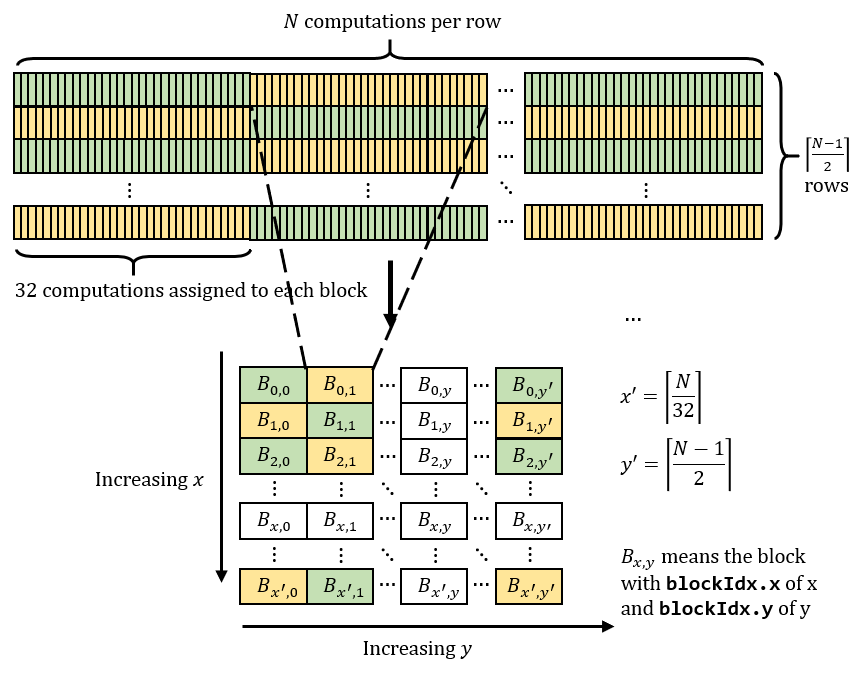
\includegraphics[width=0.9\textwidth]{reportAssets/chap32DCollisionPairMapping.png}
    \caption{Mapping of 2D computations array to 2D kernel grid}
    \label{fig:collisionMatrixMapping}
\end{figure}

\subsection{Thread Arrangement}

All our kernels are launched with grids comprising only 1D thread blocks. Hence, the arrangement of threads within a block is trivial - a thread's coordinates in its block is simply \texttt{threadIdx.x}. Excess threads are checked for and \texttt{return} immediately, performing no work.\\

For kernels \texttt{checkWallCollision} and \texttt{updateParticles}, the mapping of a thread to a particle is
\begin{itemize}
    \item \texttt{particleIdx = blockIdx.x * blockDim.x + threadIdx.x}
\end{itemize}

Similarly, for the kernel \texttt{settleCollision}, the mapping of a thread to a collision to resolve is
\begin{itemize}
    \item \texttt{collisionIdx = blockIdx.x * blockDim.x + threadIdx.x}
\end{itemize}

\pagebreak

For the kernel \texttt{checkCollision}, there are multiple cases to consider when mapping a thread to two particles \texttt{pIdx} and \texttt{qIdx}.
\begin{itemize}
    \item For each thread, compute the following temporary indices
    \begin{itemize}
        \item \texttt{pTemp = blockIdx.x}
        \item \texttt{qTemp = blockDim.x * blockIdx.y + threadIdx.x}
    \end{itemize}
    \item Full row (odd $N$ or even $N$ but block has a \texttt{blockIdx.x != (N / 2) - 1})
    \begin{itemize}
        \item If \texttt{pTemp <= qTemp}, then it is a reflected computation
        \begin{itemize}
            \item[$\bullet$] \texttt{pIdx = N - 2 - pIndex; qIdx = N - 1 - qIndex}
        \end{itemize}
        \item Otherwise, \texttt{pIdx = pTemp; qIdx = qTemp}
    \end{itemize}
    \item Leftover row (only for even $N$): block has \texttt{blockIdx.x == (N / 2) - 1}
    \begin{itemize}
        \item[$\bullet$] Only compute when \texttt{qTemp > pTemp} for $j > i$ since there are no reflected computations in this row
    \end{itemize}
\end{itemize}

\pagebreak

\section{Discussion: Floating-point Precision}

\subsection{Observations}
In our initial runs of the default testcase, we noticed that the CUDA implementation did not converge to the same final state as the OpenMP implementation. To investigate this anomaly, we re-ran the default testcase in \texttt{print} mode and observed that differences in the floating-point (FP) position of particles manifested as early as the first time step.

\subsection{GPU Floating-point Computations}
\label{subsection:gpu-floating-point}
We read the report on \textit{Floating Point and IEEE 754 Compliance for Nvidia GPUs}, published by Nvidia in 2011 \cite{floatingCompliance}. Of particular significance are the following details on FP computations in general:
\begin{enumerate}
    \item The IEEE 754 standard specifies a common encoding for basic FP formats for consistency across platforms. It also recommends extended FP formats, but does not specify any particular implementation.
    \begin{itemize}
        \item Single-precision (FP32): 1-bit sign, 8-bit exponent, 23-bit significand
        \item Double-precision (FP64): 1-bit sign, 12-bit exponent, 53-bit significand
    \end{itemize}
    \item Due to its finite precision, FP arithmetic violates the rules and properties of mathematical arithmetic. The order of execution of basic FP operations influences the accuracy of the final result, due to rounding of intermediate values to a specified precision.
    \begin{itemize}
        \item Violation of \textbf{associativity}: Mathematically, $(A + B) + C = A + (B + C)$, but $rn(rn(A + B) + C) \neq rn(A + rn(B + C))$ for FP arithmetic (here, $rn$ rounds the result)
    \end{itemize}
    \item The IEEE 754 standard also specifies a \textit{fused-multiply add} (FMA) operation, which computes the result of $rn(A \times B + C)$ with only one rounding operation.
    \begin{itemize}
        \item Using the FMA operation results in greater accuracy as compared to computing $rn(rn(A \times B) + C)$, which requires two rounding operations
    \end{itemize}
    \item \textbf{Subtractive cancellation}: Addition of two FP numbers with similar magnitudes but different signs result in a loss in precision, as many of the leading bits cancel, leaving fewer bits of precision in the final result. However, this can be avoided using the FMA operation.
    \begin{itemize}
        \item The FMA operation first computes a double-width product $A \times B$ during the multiplication, i.e. if $A, B$ are FP64 numbers, then $A \times B$ is a FP128 number
        \item $A \times B$ thus has a 106-bit significand, whilst $C$ has a 53-bit significand
        \item Therefore, even if subtractive cancellation occurs during the addition of $(A \times B)$ and $C$, there remains at least 53 valid bits of precision, resulting in no loss of precision in the final result
    \end{itemize}
    \item Nvidia GPUs provide native hardware support for both FP32 and FP64 FMA operations, and using them is faster and more accurate than performing separate multiply and add operations.
    \item By default, the Nvidia CUDA compiler (NVCC) optimises CUDA programs by merging successive FP multiply and add operations into FMA operations.
    \begin{itemize}
        \item This FMA merging optimisation may be explicitly disabled by using the CUDA compiler flag \texttt{--fmad=false}
    \end{itemize}
    \item There is no standardised accuracy level for FP mathematical functions implemented by different libraries. Functions compiled for the host (\texttt{\_\_host\_\_} functions) use the host compiler's math library whereas functions compiled for the device, i.e. \texttt{\_\_global\_\_} and \texttt{\_\_device\_\_} functions, use the CUDA math library implementation.
    \begin{itemize}
        \item Since we make use of the \texttt{sqrt} function when checking particle-particle collisions, this introduces deviations between our OpenMP and CUDA implementations
    \end{itemize} 
\end{enumerate}

\subsection{Floating-point Hardware Comparison}
The hardware support for double-precision FP64 numbers and FP operations also differ between modern CPUs (that support the AMD64 ISA) and GPUs.
\begin{enumerate}
    \item CPUs possess 64-bit GPRs, whereas many GPUs only possess 32-bit registers. Therefore, whilst CPUs store FP64 numbers in a single GPR, GPUs store FP64 numbers in a pair of adjacent registers.
    \item CPUs have specialised FP units (FPUs) as coprocessors for performing scalar and vector FP64 computations natively.
    \begin{itemize}
        \item Scalar FP64 operations (specifically x87 instructions) are performed with an 80-bit extended precision format to minimise precision loss from overflow and rounding of intermediate values, before the results are rounded and stored in GPRs
        \item Vector FP64 operations are performed on extra-wide registers (albeit at lower precision than x87 instructions), via support for one or more of the following supplementary instruction sets: \textit{Advanced Vector Extensions} (AVX) or \textit{Streaming SIMD Extensions} (SSE)
        \begin{itemize}
            \item These extensions also provide instructions for scalar FP64 operations on extra-wide XMM registers
        \end{itemize}
        \item Some CPUs also possess hardware support for FMA operations, by providing an FMA instruction from the FMA instruction set to compilers
    \end{itemize}
    \item In contrast, GPUs emulate FP64 operations by decomposing them into a sequence of instructions (\textit{subroutines}) on pairs of 32-bit registers, that are only performed by the FP64 units within each SM.
    \begin{itemize}
        \item Consumer-grade Nvidia CPUs only possess two hardware FP64 units per SM, primarily to ensure that CUDA programs with FP64 code operates correctly (but not necessarily quickly) \cite{turingarchi}
        \begin{itemize}
            \item Thus, the throughput of FP64 instructions suffers heavily relative to FP32 instructions - for the Titan RTX and Tesla T4, the FP64 instruction throughput is $\frac{1}{32}$ that of its FP32 instruction throughput
        \end{itemize}
        \item Datacentre-grade Nvidia GPUs possess the full 32 hardware FP64 units per SM, allowing them to run CUDA programs with FP64 code with no performance loss
        \begin{itemize}
            \item Since one FP64 number requires two registers to be stored, the final throughput of FP64 instructions is only half that of FP32 instructions
            \item Amongst the GPU nodes in the Compute Cluster, only the Tesla V100 and Titan V have this 2:1 ratio of FP32 to FP64 TFLOPS throughput
        \end{itemize}
    \end{itemize}
\end{enumerate}

\subsection{Divergence Results}
To investigate the rate at which the simulation state diverged, we ran the default testcase in \texttt{print} mode for both implementations. Additionally, the CUDA implementation was ran once with the flag \texttt{--fmad=true} and once with \texttt{--fmad=false}, to explicitly enable or disable the FMA merging optimisation respectively.\\

We used the simulation state of the OpenMP implementation as a reference, and considered the state of a particle to have \textit{diverged} at a time step $S$ if at least one of $x, y, v_x$ or $v_y$ differed at the 8\textsuperscript{th} decimal position.\\

Figure \ref{fig:divergedParticles} below plots the number of diverged particles $N_{div}$ against the step number $S$. Note that the horizontal axis only displays $S$ to 180 instead of the full 1000 steps for the default testcase.\\

\begin{figure}[H]
    \centering
    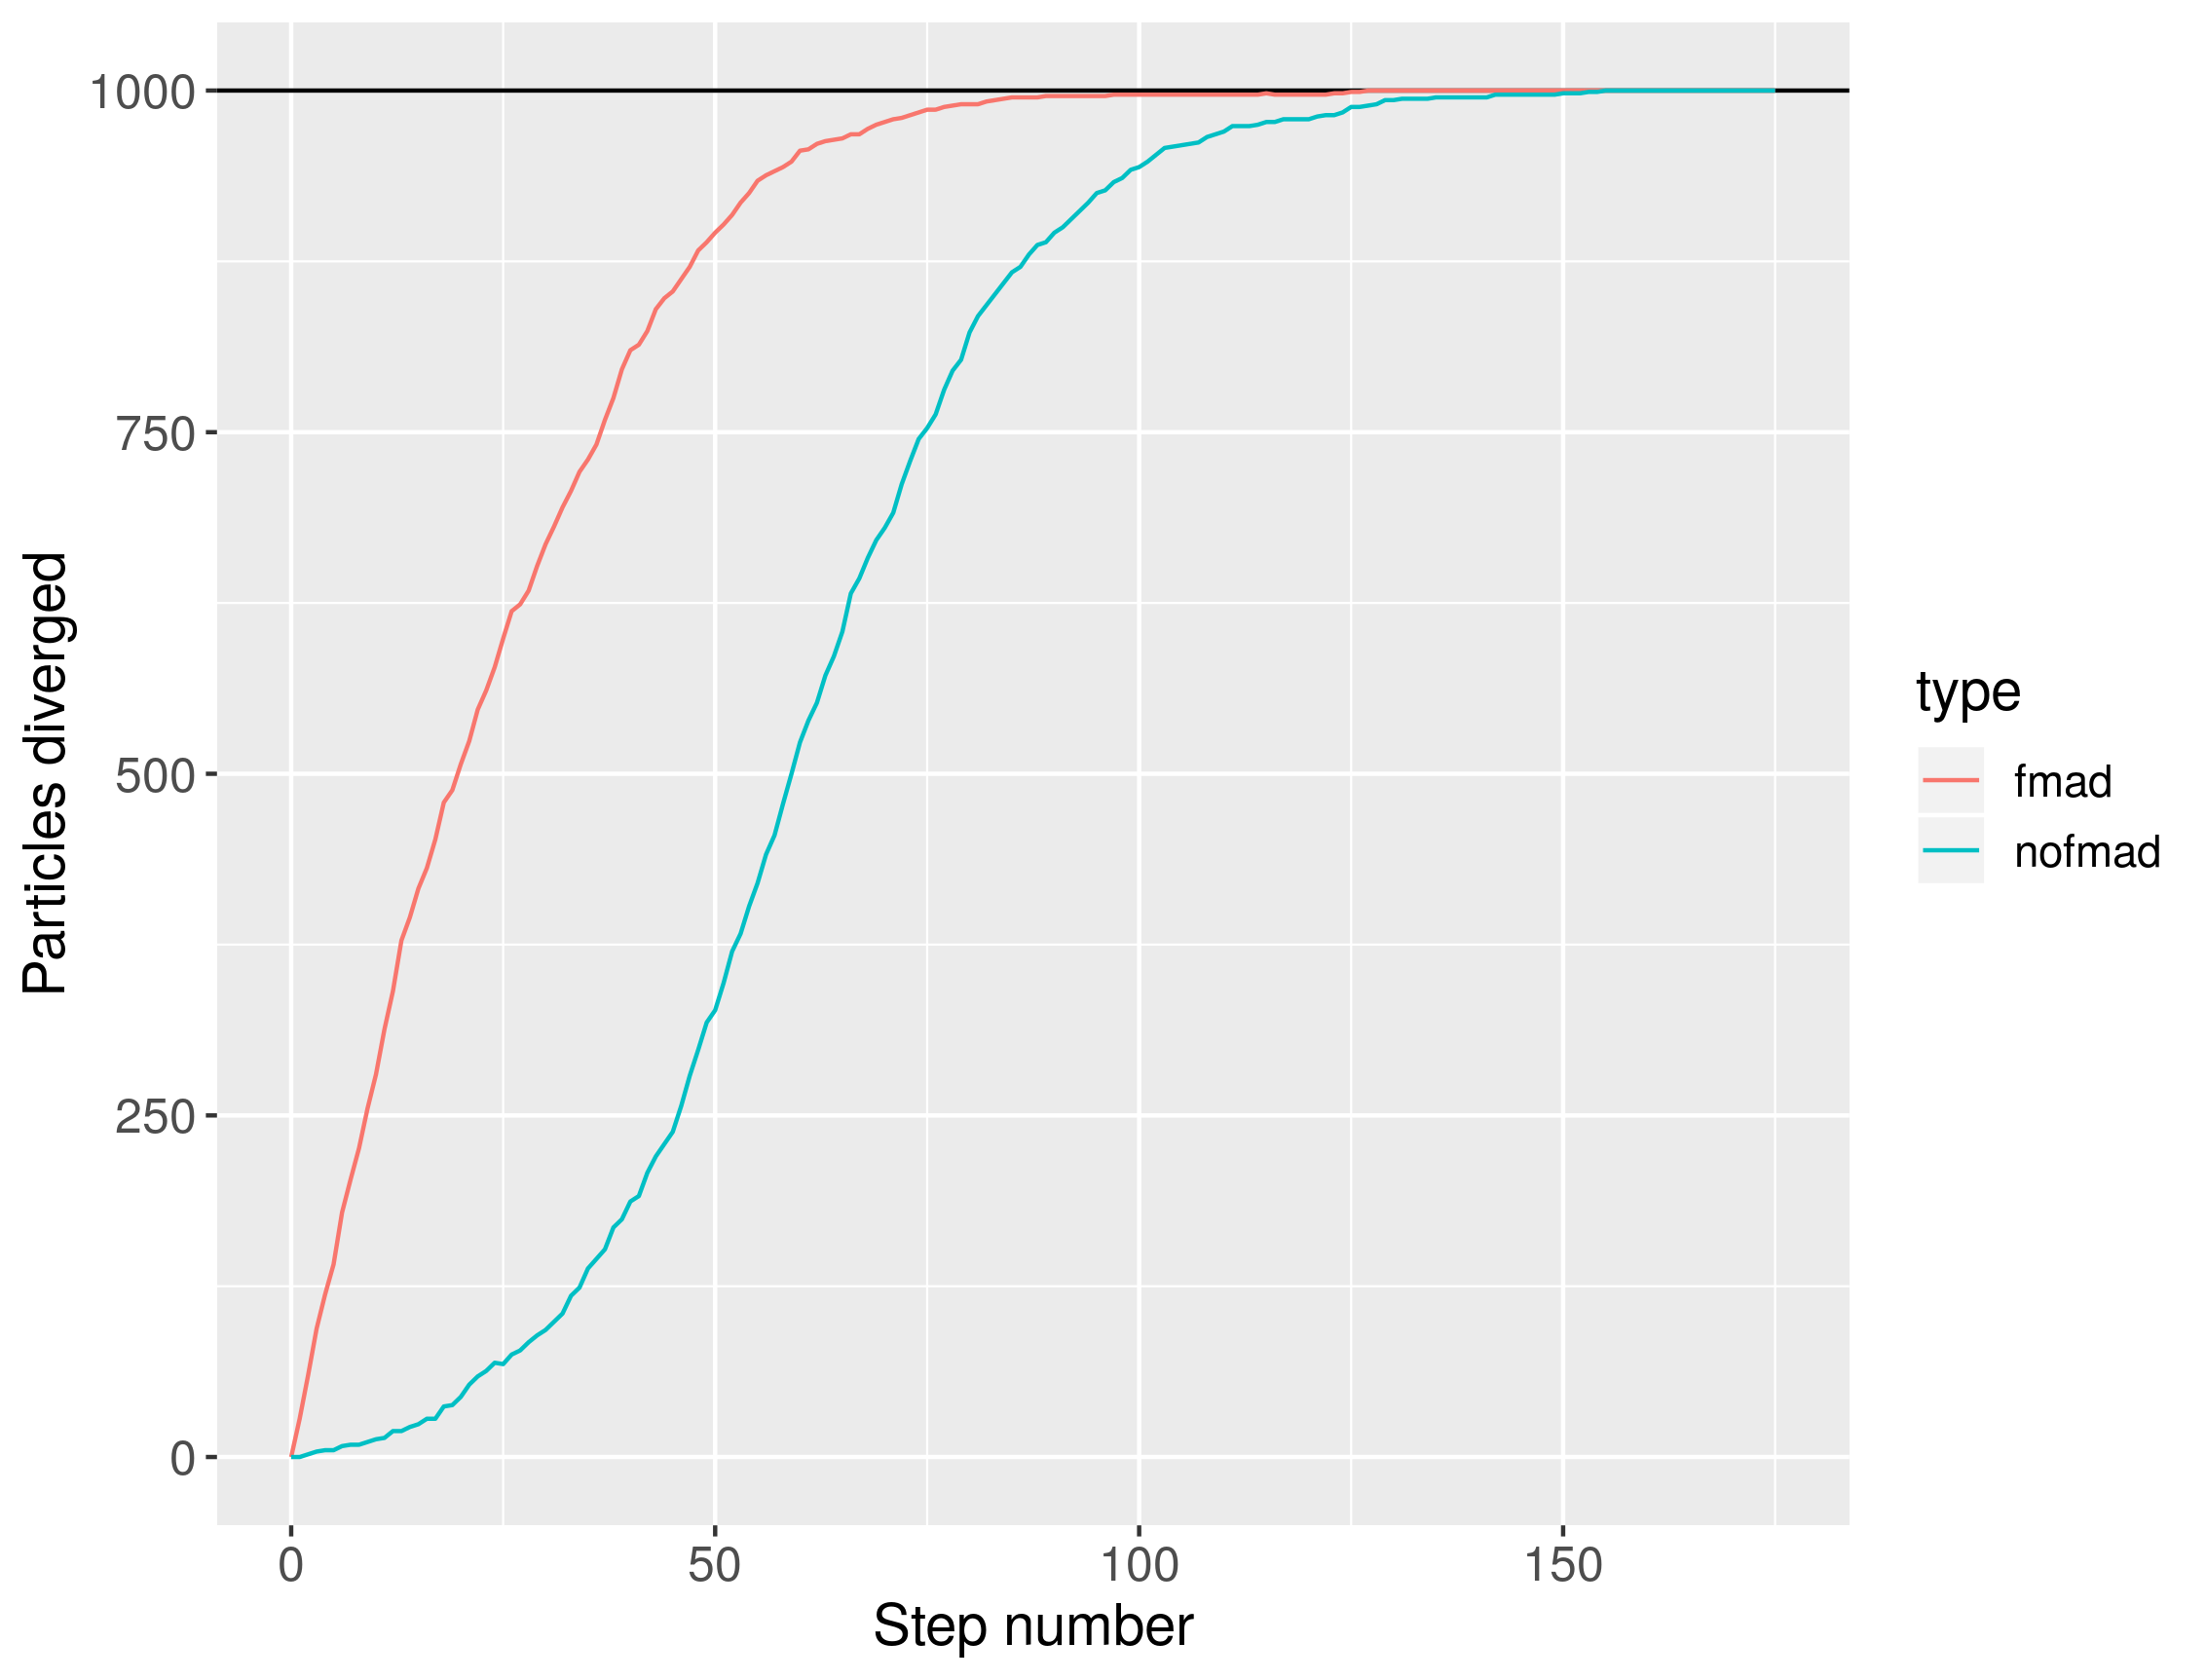
\includegraphics[width=0.9\textwidth]{divergedParticles}
    \caption{Plot of number of incorrect particles against time step}
    \label{fig:divergedParticles}
\end{figure}

\subsection{Correctness}

Figure \ref{fig:divergedParticles} shows that enabling the FMA merging optimisation leads to a faster divergence of the simulation state from the OpenMP implementation, with full divergence occurring at $S=127$ as compared to $S=155$. This demonstrates that discrete particle simulation is highly sensitive to small perturbations in the simulation state, with the large degree of chaos making it difficult to ascertain correctness.\\

Suppose we treat the simulation results from the OpenMP implementation as the ``\textit{correct}" result, then this runs counter to our expectation that the FMA operation is more numerically precise than separate FP multiply and add operations. Leaving the FMA optimisation enabled \textit{should} result in better agreement with the intermediate simulation states of the OpenMP implementation, but this is not observed.\\

We inspected the assembly output of our OpenMP implementation, and found that the C compiler output scalar FP64 SSE2 instructions, without any higher-precision x87 or FMA instructions.\\

Reading the documentation of the GNU Compiler Collection (GCC) C compiler that is invoked by NVCC, we find that by default, the compiler \textbf{does not} generate vector or FMA instructions even if supported by the underlying hardware. Vector and FMA instructions must be specifically enabled with the sequence of compiler flags \texttt{-O2 -mavx2 -mfma}.\\

Despite re-compiling the OpenMP implementation with these flags and running the default testcase again, the simulations still exhibited rapid divergence that was complete at about $S = 150$. Given the numerous differences between the mode of FP computations between CPUs and GPUs, we conclude that there is no deterministic way to determine correctness of either implementation. We recommend that visual inspection of the simulation state at every step be employed instead.

\pagebreak

\section{Test Conditions and Testcases}

\subsection{Test Setup}

For ease of deployment, we wrote a Bash script to automate the compilation, test case generation, profiling and transfer of results back to Sunfire with different sets of source code. The scripts can be found in the folder \texttt{/testDispatcher}.\\

Benchmarking of our previous OpenMP (parallel) implementation was done on the Intel Xeon Silver 4114 node, specifically \ul{soctf-pdc-010}. We ran the program on 20 threads, which we found to produce the highest speedup with respect to our sequential implementation. \cite{assignref}\\

Benchmarking of our CUDA implementations was done on the Compute Cluster nodes, specifically node \ul{xgpe1} with two Xeon Silver 4116 CPUs and a Nvidia Titan RTX GPU, and node \ul{xgpf1} with two Xeon Silver 4116 CPUs and a Nvidia Tesla T4 GPU.\\

The CUDA implementations were also benchmarked on the Jetson TX2 node, specifically \ul{jetsontx2-01}. However, due to the excessively long runtime for small testcases, the larger testcases with $N > 6000$ were skipped.\\

A Python script was used to generate the input files for each of the implementations. Each testcase was run five times and the fastest execution time was retained as the datapoint for that testcase.\\

To replicate our results for a given implementation, run \bt{./test.sh} in the particular implementation's folder. It is recommended to change the target folder for the \bt{scp} command as it will automatically transfer all the results out when it is complete.

\subsection{Random Testcases}
\label{section:random-testcases}

For benchmarking, testcases ran in \textit{perf} mode and the initial states of particles were not provided. Variables of the simulation were adjusted for each testcase.\\

The simulation parameters of the default testcase are
\begin{itemize}
	\item $N = 1000, L=20000, r=1, S=1000$
\end{itemize}

The testcases that were executed for each implementation are as follows.
\begin{enumerate}
	\item CPU (parallel) implementation - 20 OpenMP threads
	\begin{itemize}
		\item Varying $N$ only: $N = 1k, 2k, 3k, 4k, 6k, 8k, 12k, 16k, 24k, 32k$
	\end{itemize}
	
	\item GPU implementation (Jetson TX2)
	\begin{itemize}
		\item $F$ = \texttt{--fmad} compile flag
		\item Varying both $N$ and $F$ together
		\begin{itemize}
			\item $N = 1k, 2k, 3k, 4k, 6k$
			\item $F =$ \texttt{true, false}
		\end{itemize}
	\end{itemize}
	
	\item GPU implementation (Nvidia Titan RTX \& Nvidia Tesla T4)
	\begin{itemize}
		\item $F$ = \texttt{--fmad} compile flag
		\item Varying both $N$ and $F$ together
		\begin{itemize}
			\item $N = 1k, 2k, 3k, 4k, 6k, 8k, 12k, 16k, 24k, 32k$
			\item $F =$ \texttt{true, false}
		\end{itemize}
	\end{itemize}
\end{enumerate}

\pagebreak

\section{Execution Results}

All plots were generated with the help of R. Some of the plots are not reproduced here for brevity.\\

The processed data is available in the submission as \texttt{.csv} files in \texttt{/data/gpu}. Raw data files from the \bt{time} and \bt{nvprof} command are available in \texttt{/data/gpu/<GPUtype>} as text files with \texttt{.time} extension and no extension respectively. The \bt{time} command was used in place of \bt{perf stat} on the Compute Cluster nodes since it was not available - however, the wall-clock time reported by both do agree.\\

All mentions of \textit{speedup} of the CUDA implementation in this section is made with reference to the execution time of the OpenMP implementation with $20$ threads, since running the large testcases on the purely sequential implementation would take too long.\\

\begin{figure}[H]
    \centering
    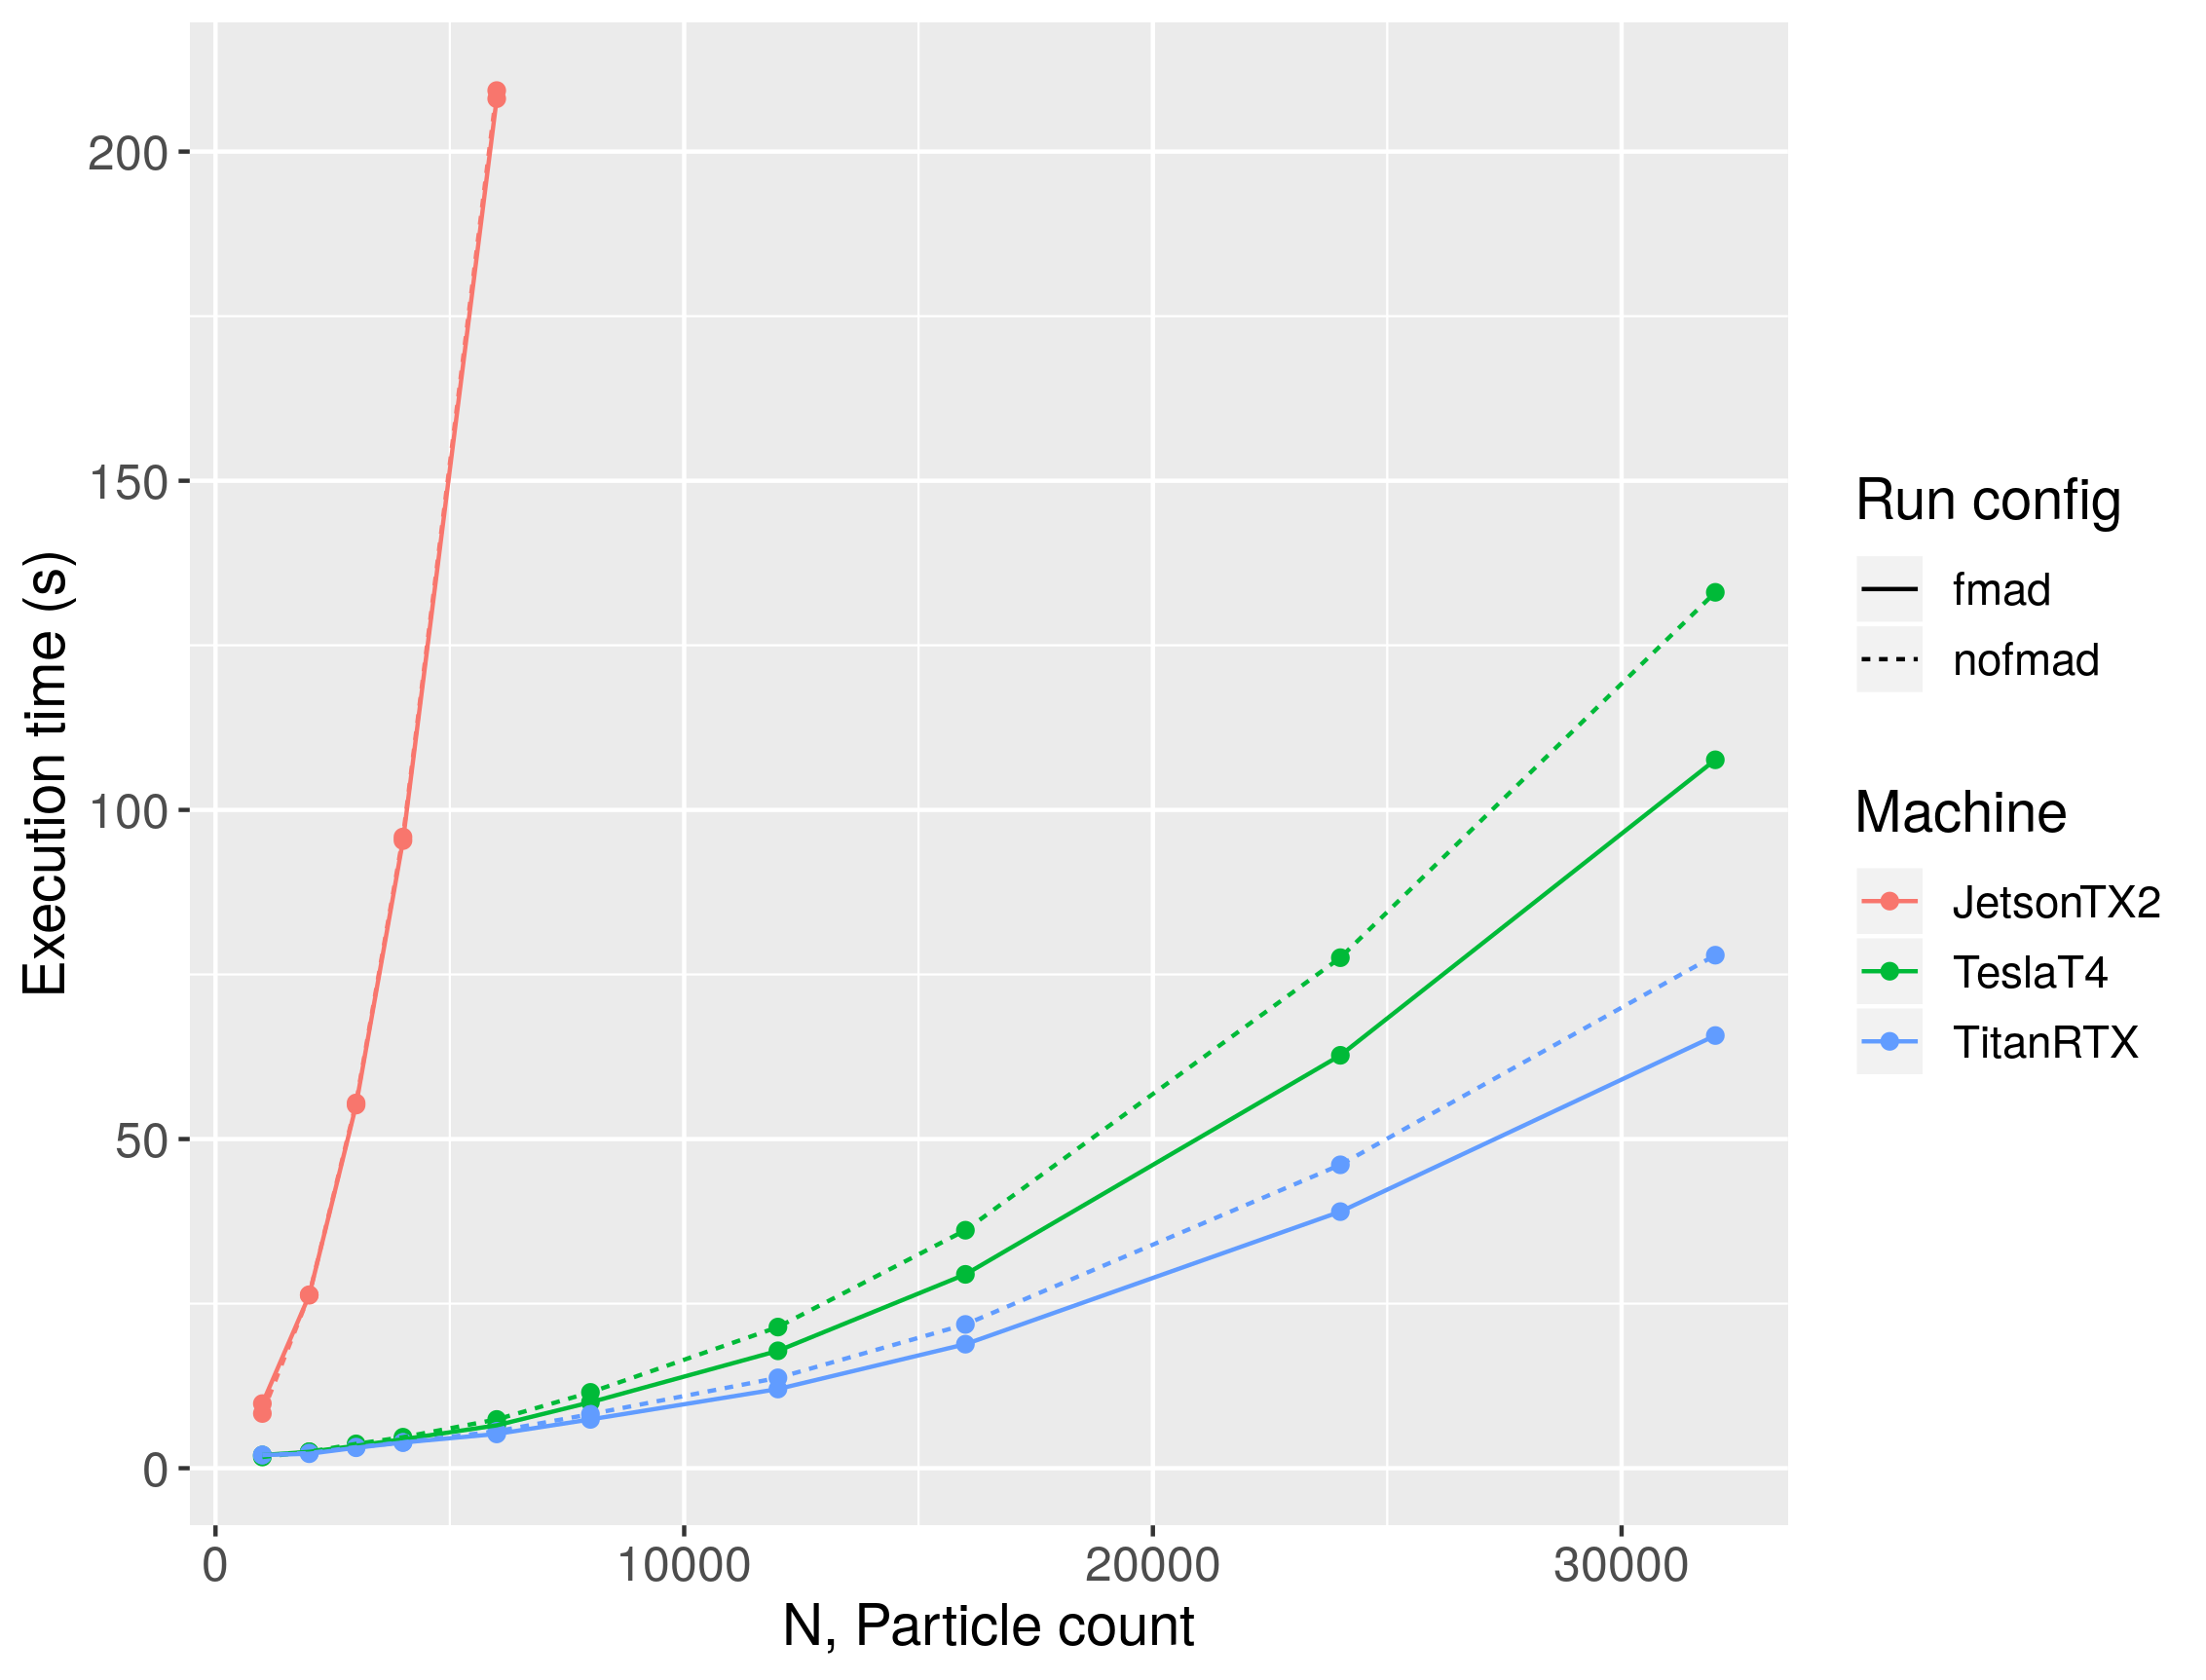
\includegraphics[width=0.75\textwidth]{gpu-varyN-withJetson}
    \caption{Plot of execution time against particle count, $N$ (including Jetson-TX2)}
    \label{fig:gpu-varyN-withJetson}
\end{figure}

\begin{figure}[H]
    \centering
    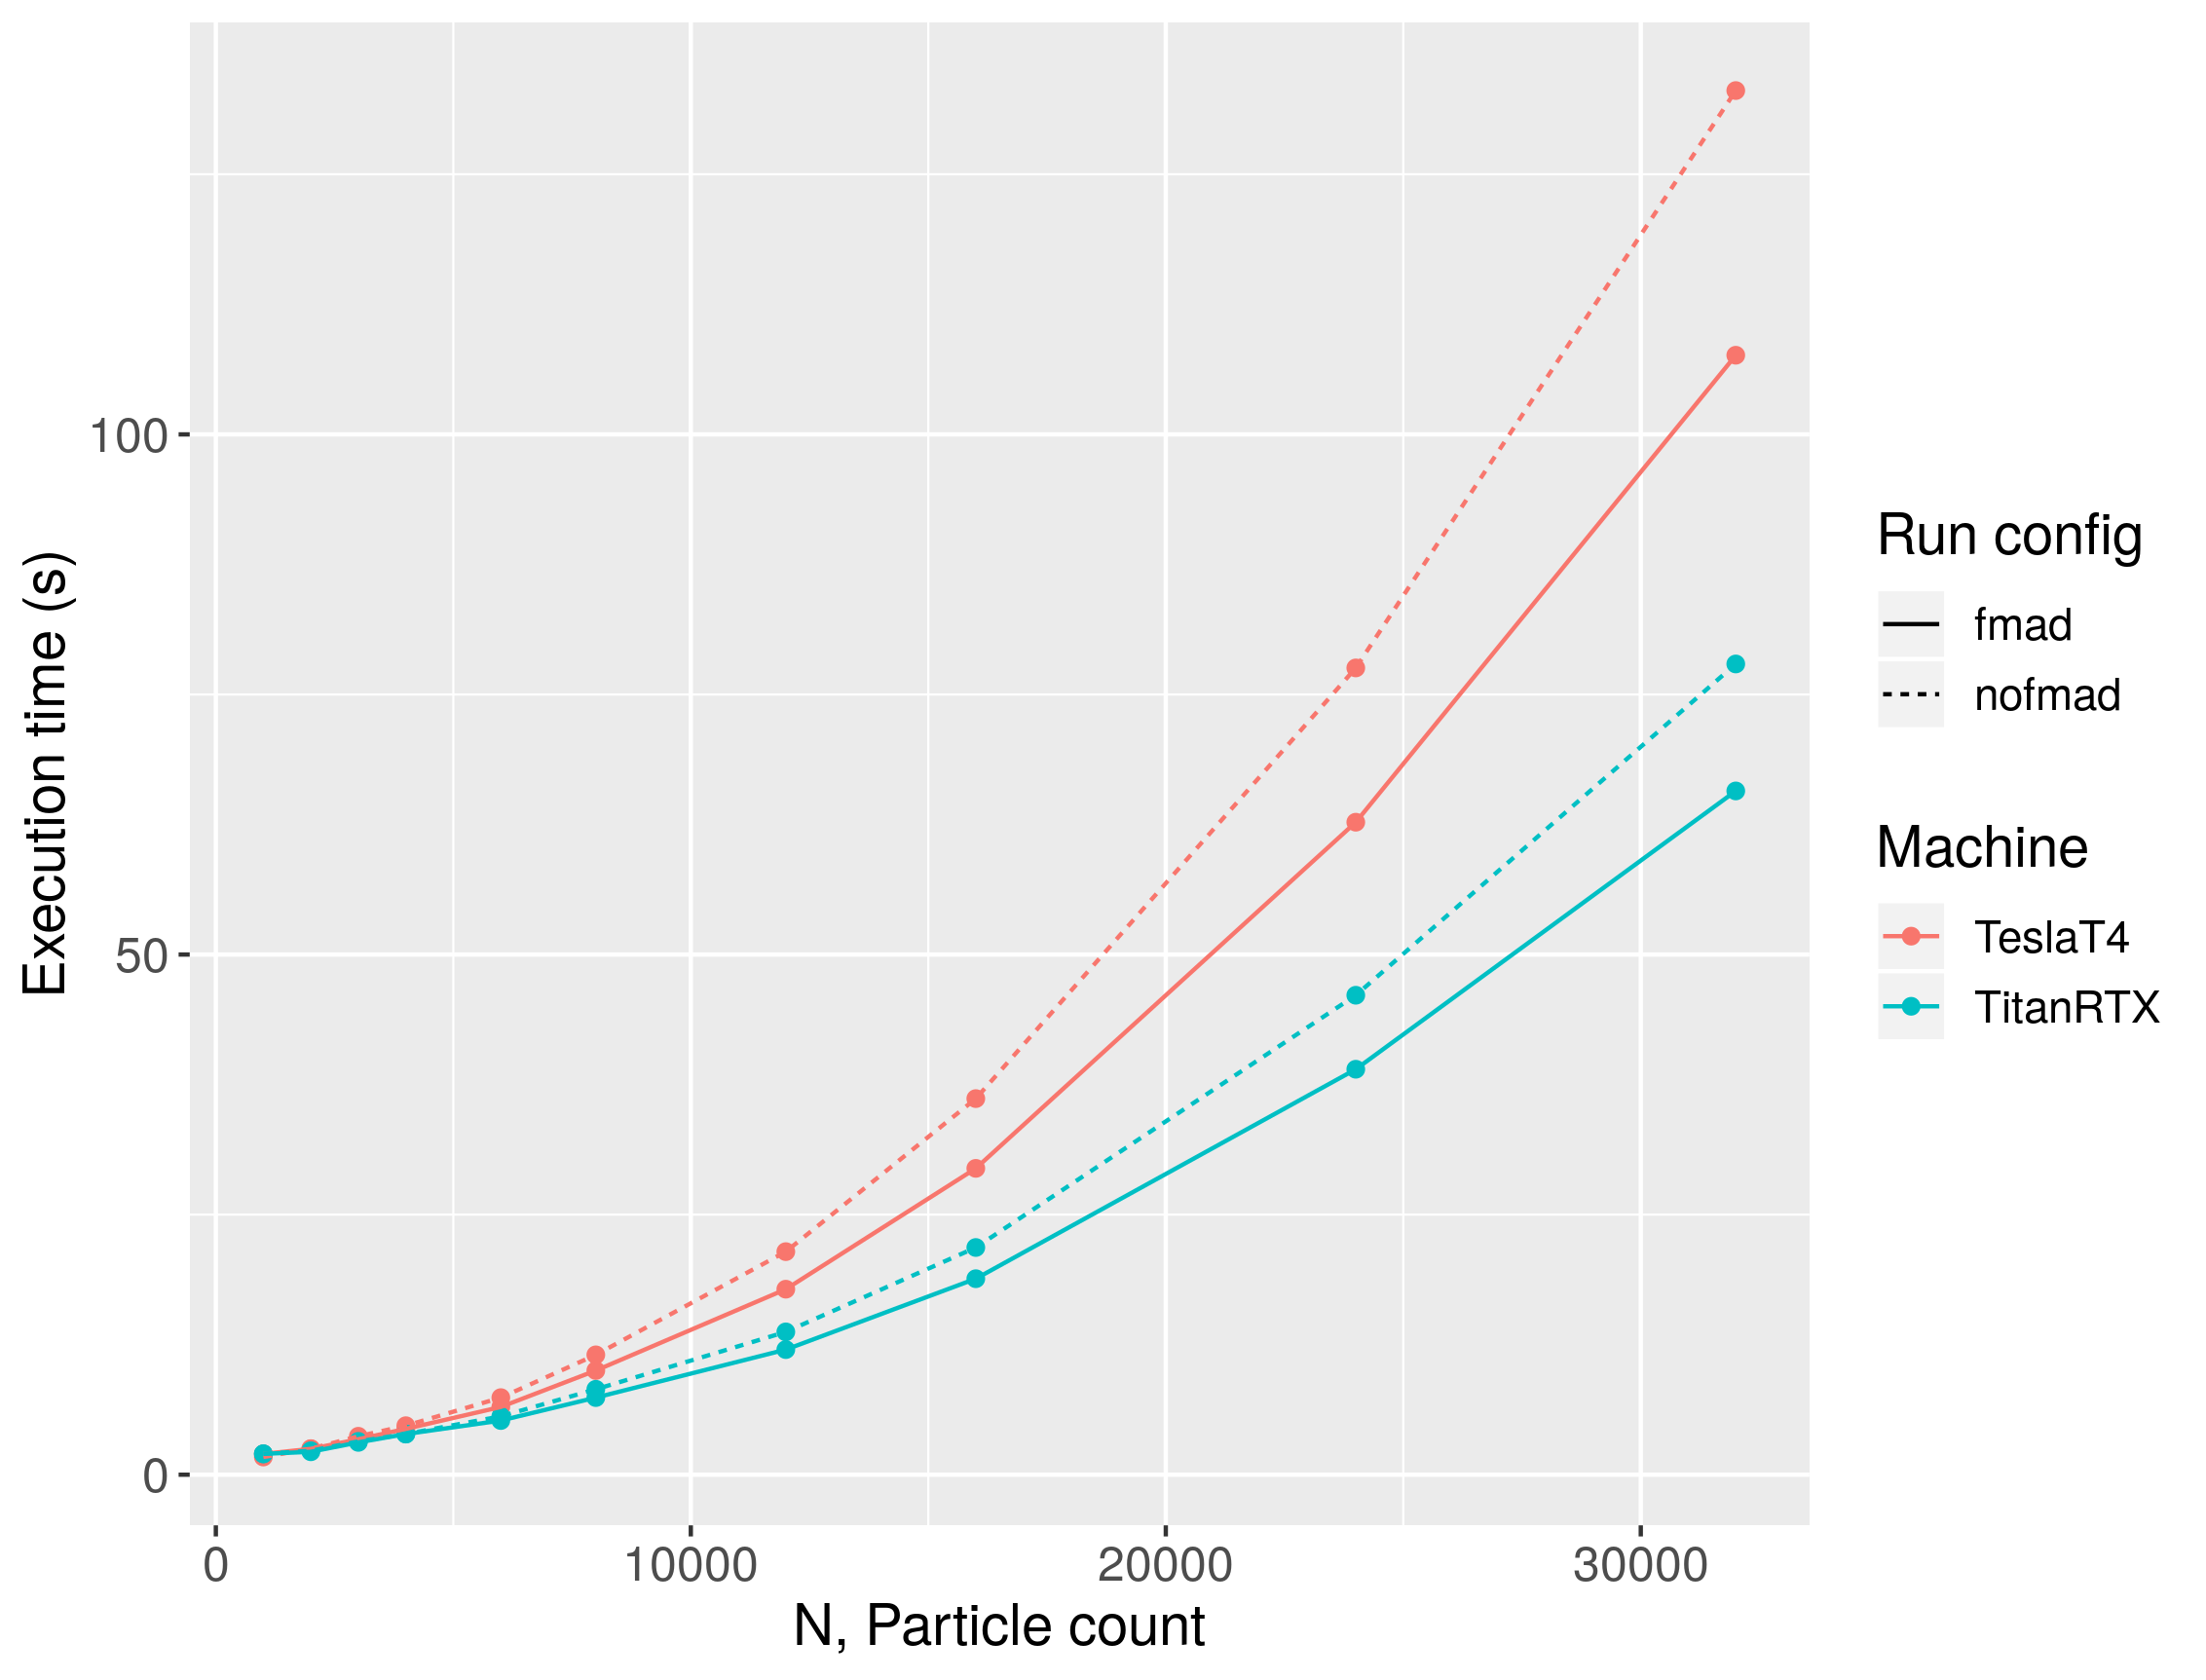
\includegraphics[width=0.75\textwidth]{gpu-varyN}
    \caption{Plot of execution time against particle count, $N$}
    \label{fig:gpu-varyN}
\end{figure}

\begin{figure}[H]
    \centering
    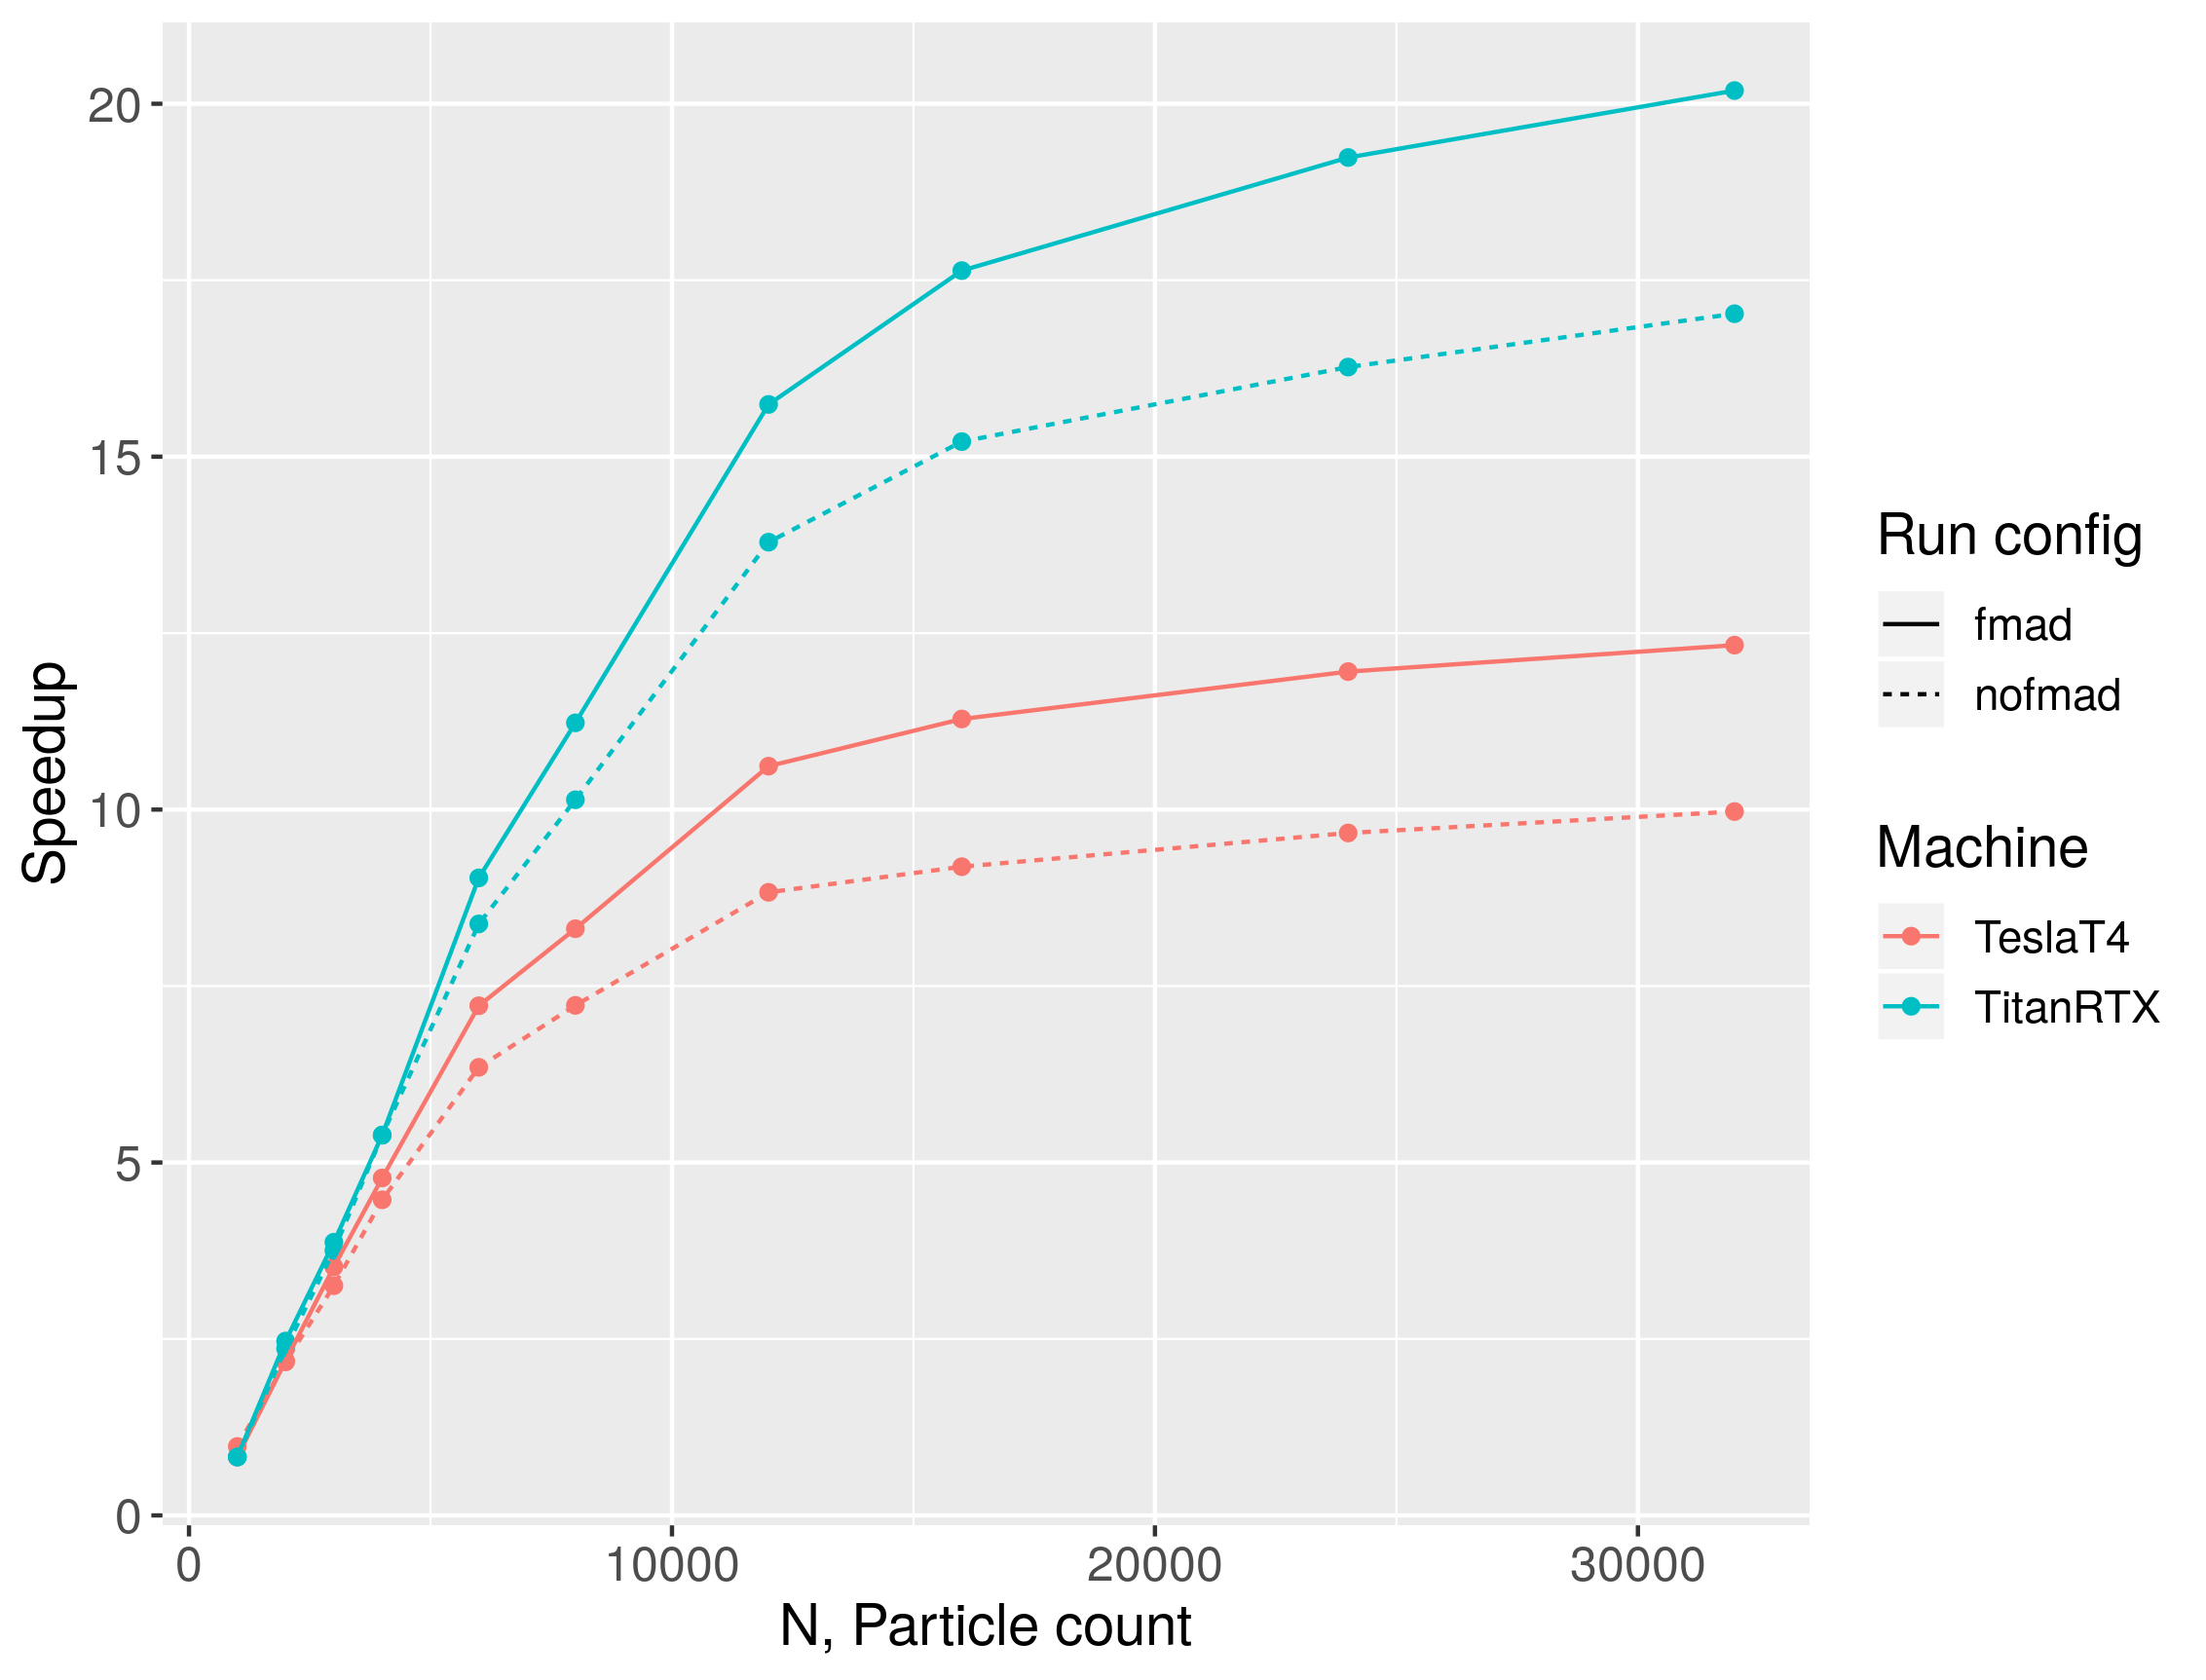
\includegraphics[width=0.75\textwidth]{gpu-speedup}
    \caption{Plot of speedup against particle count, $N$}
    \label{fig:gpu-speedup}
\end{figure}

\begin{figure}[H]
    \centering
    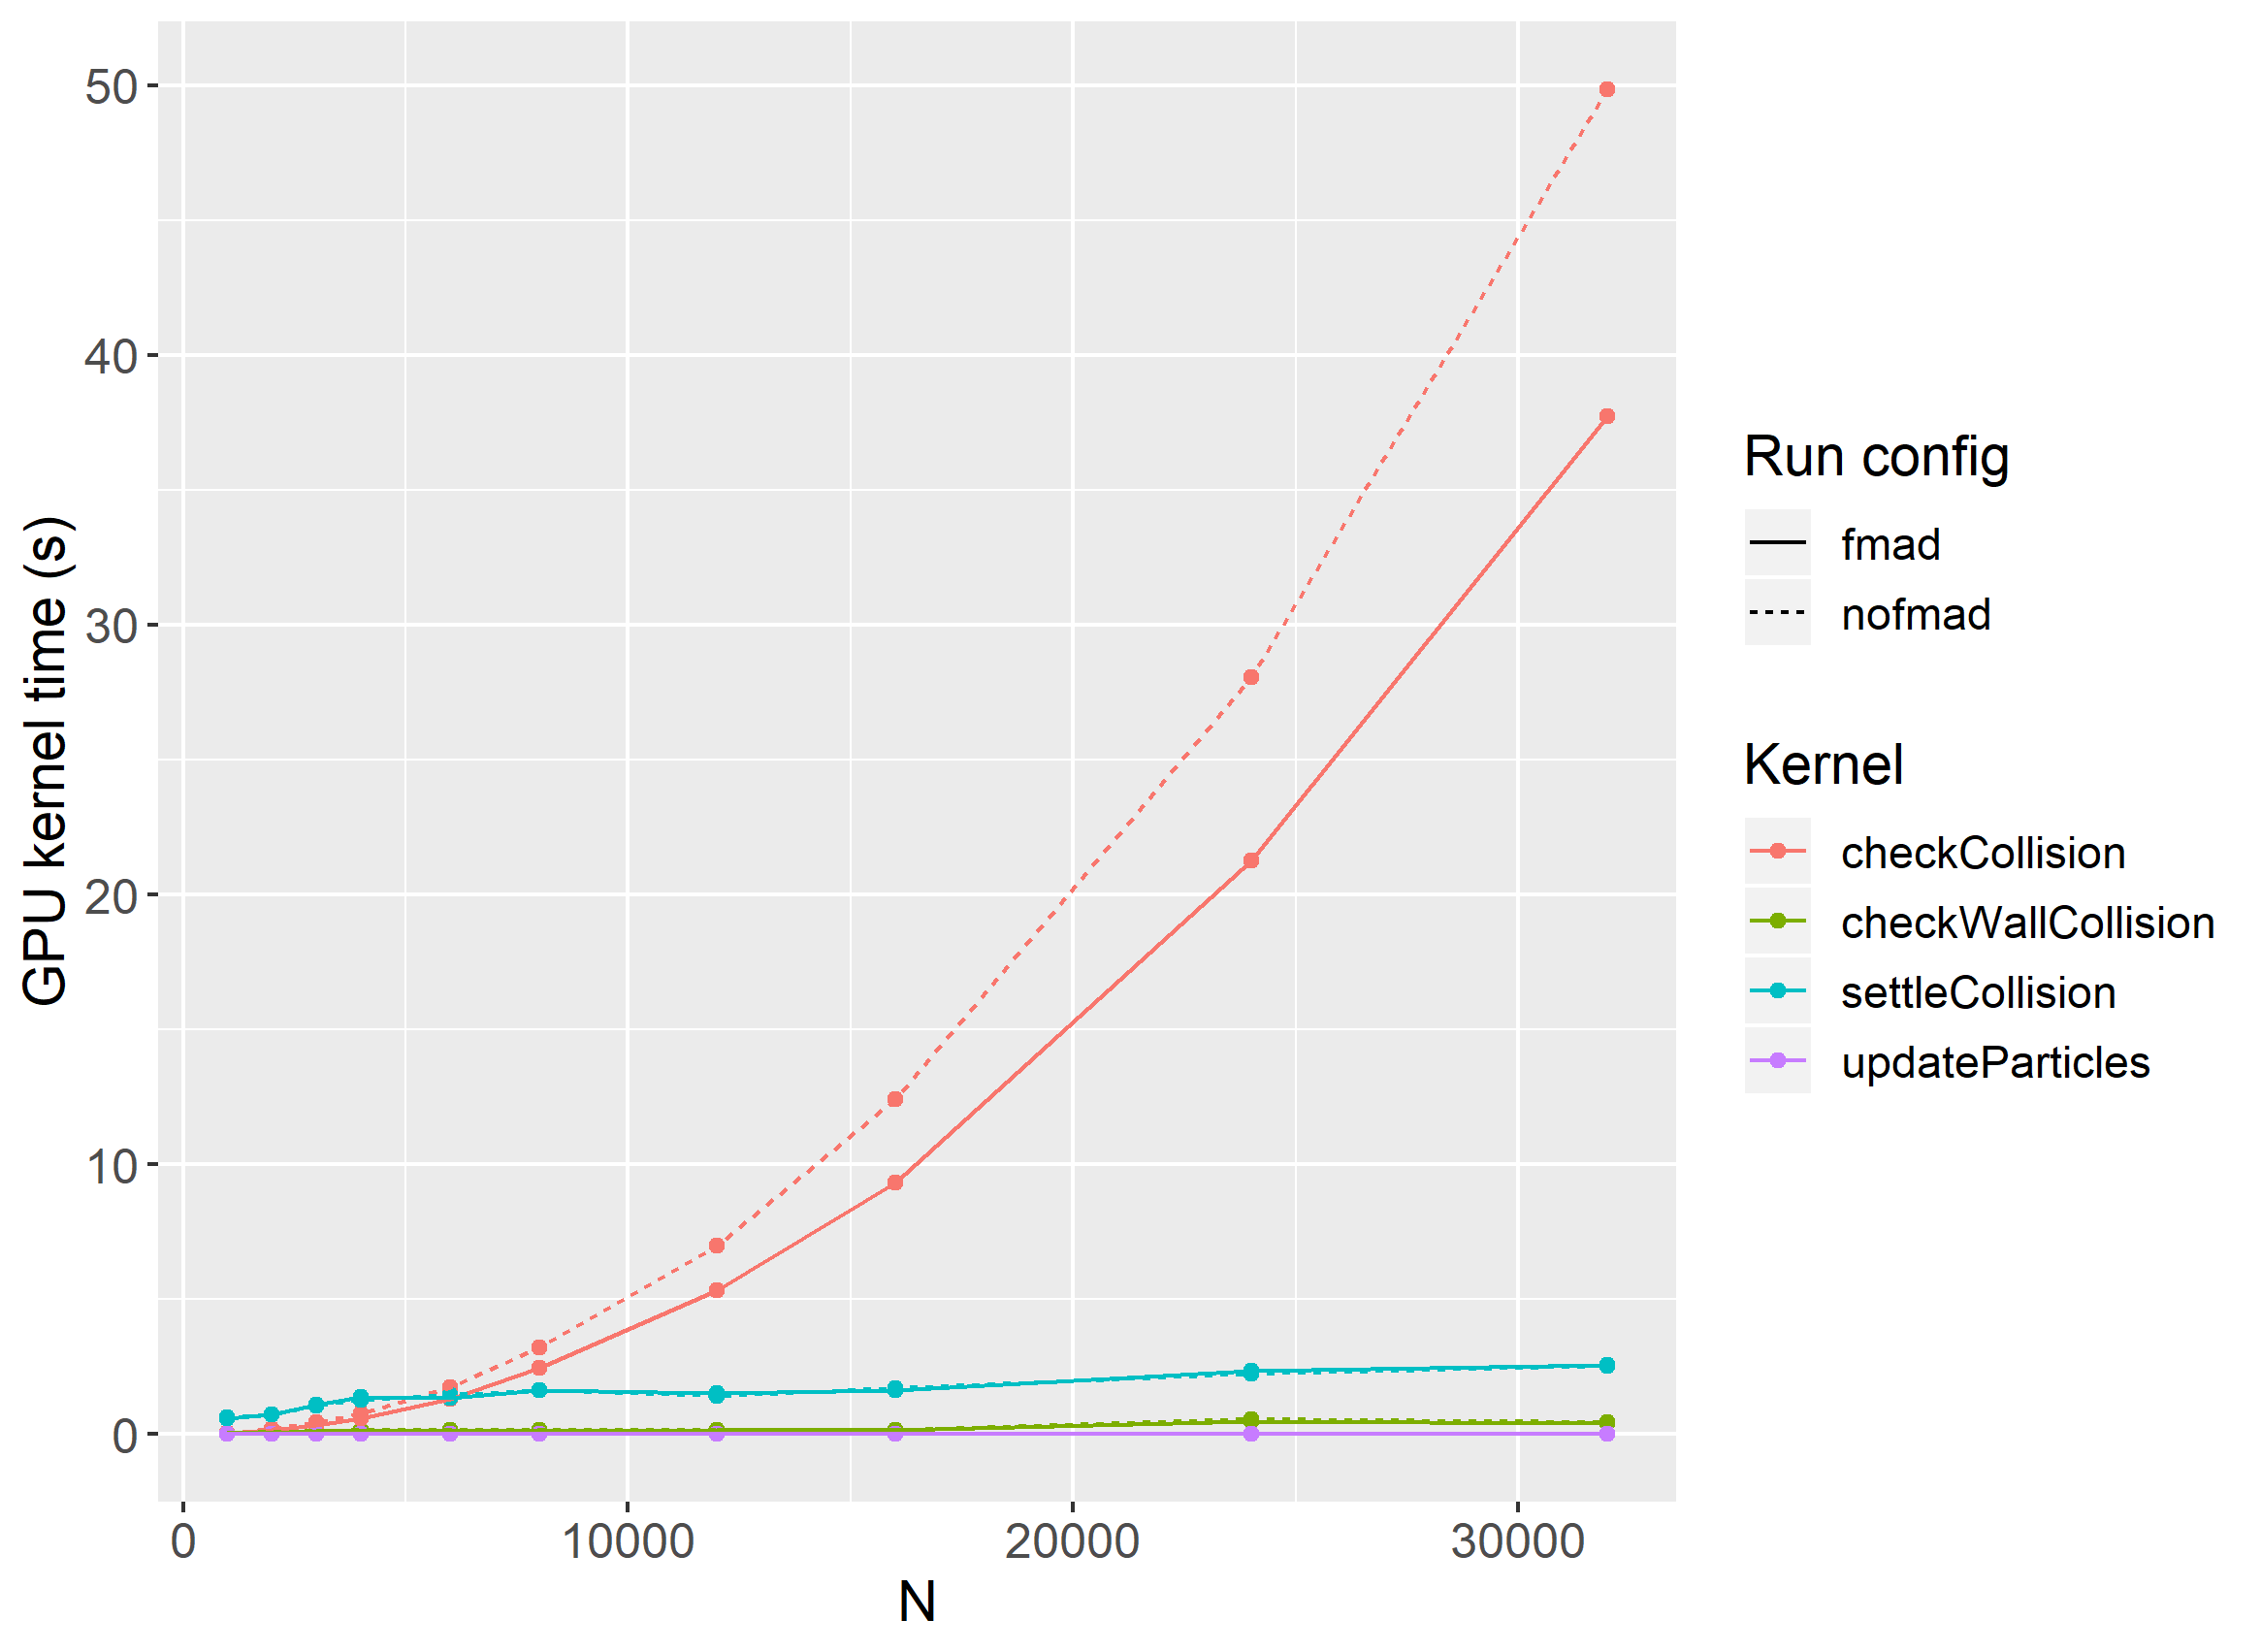
\includegraphics[width=0.75\textwidth]{titan-fmad-kernelTime-all}
    \caption{Plot of kernel time against $N$ (all kernels)}
    \label{fig:titan-fmad-kernelTime-all}
\end{figure}

\begin{figure}[H]
    \centering
    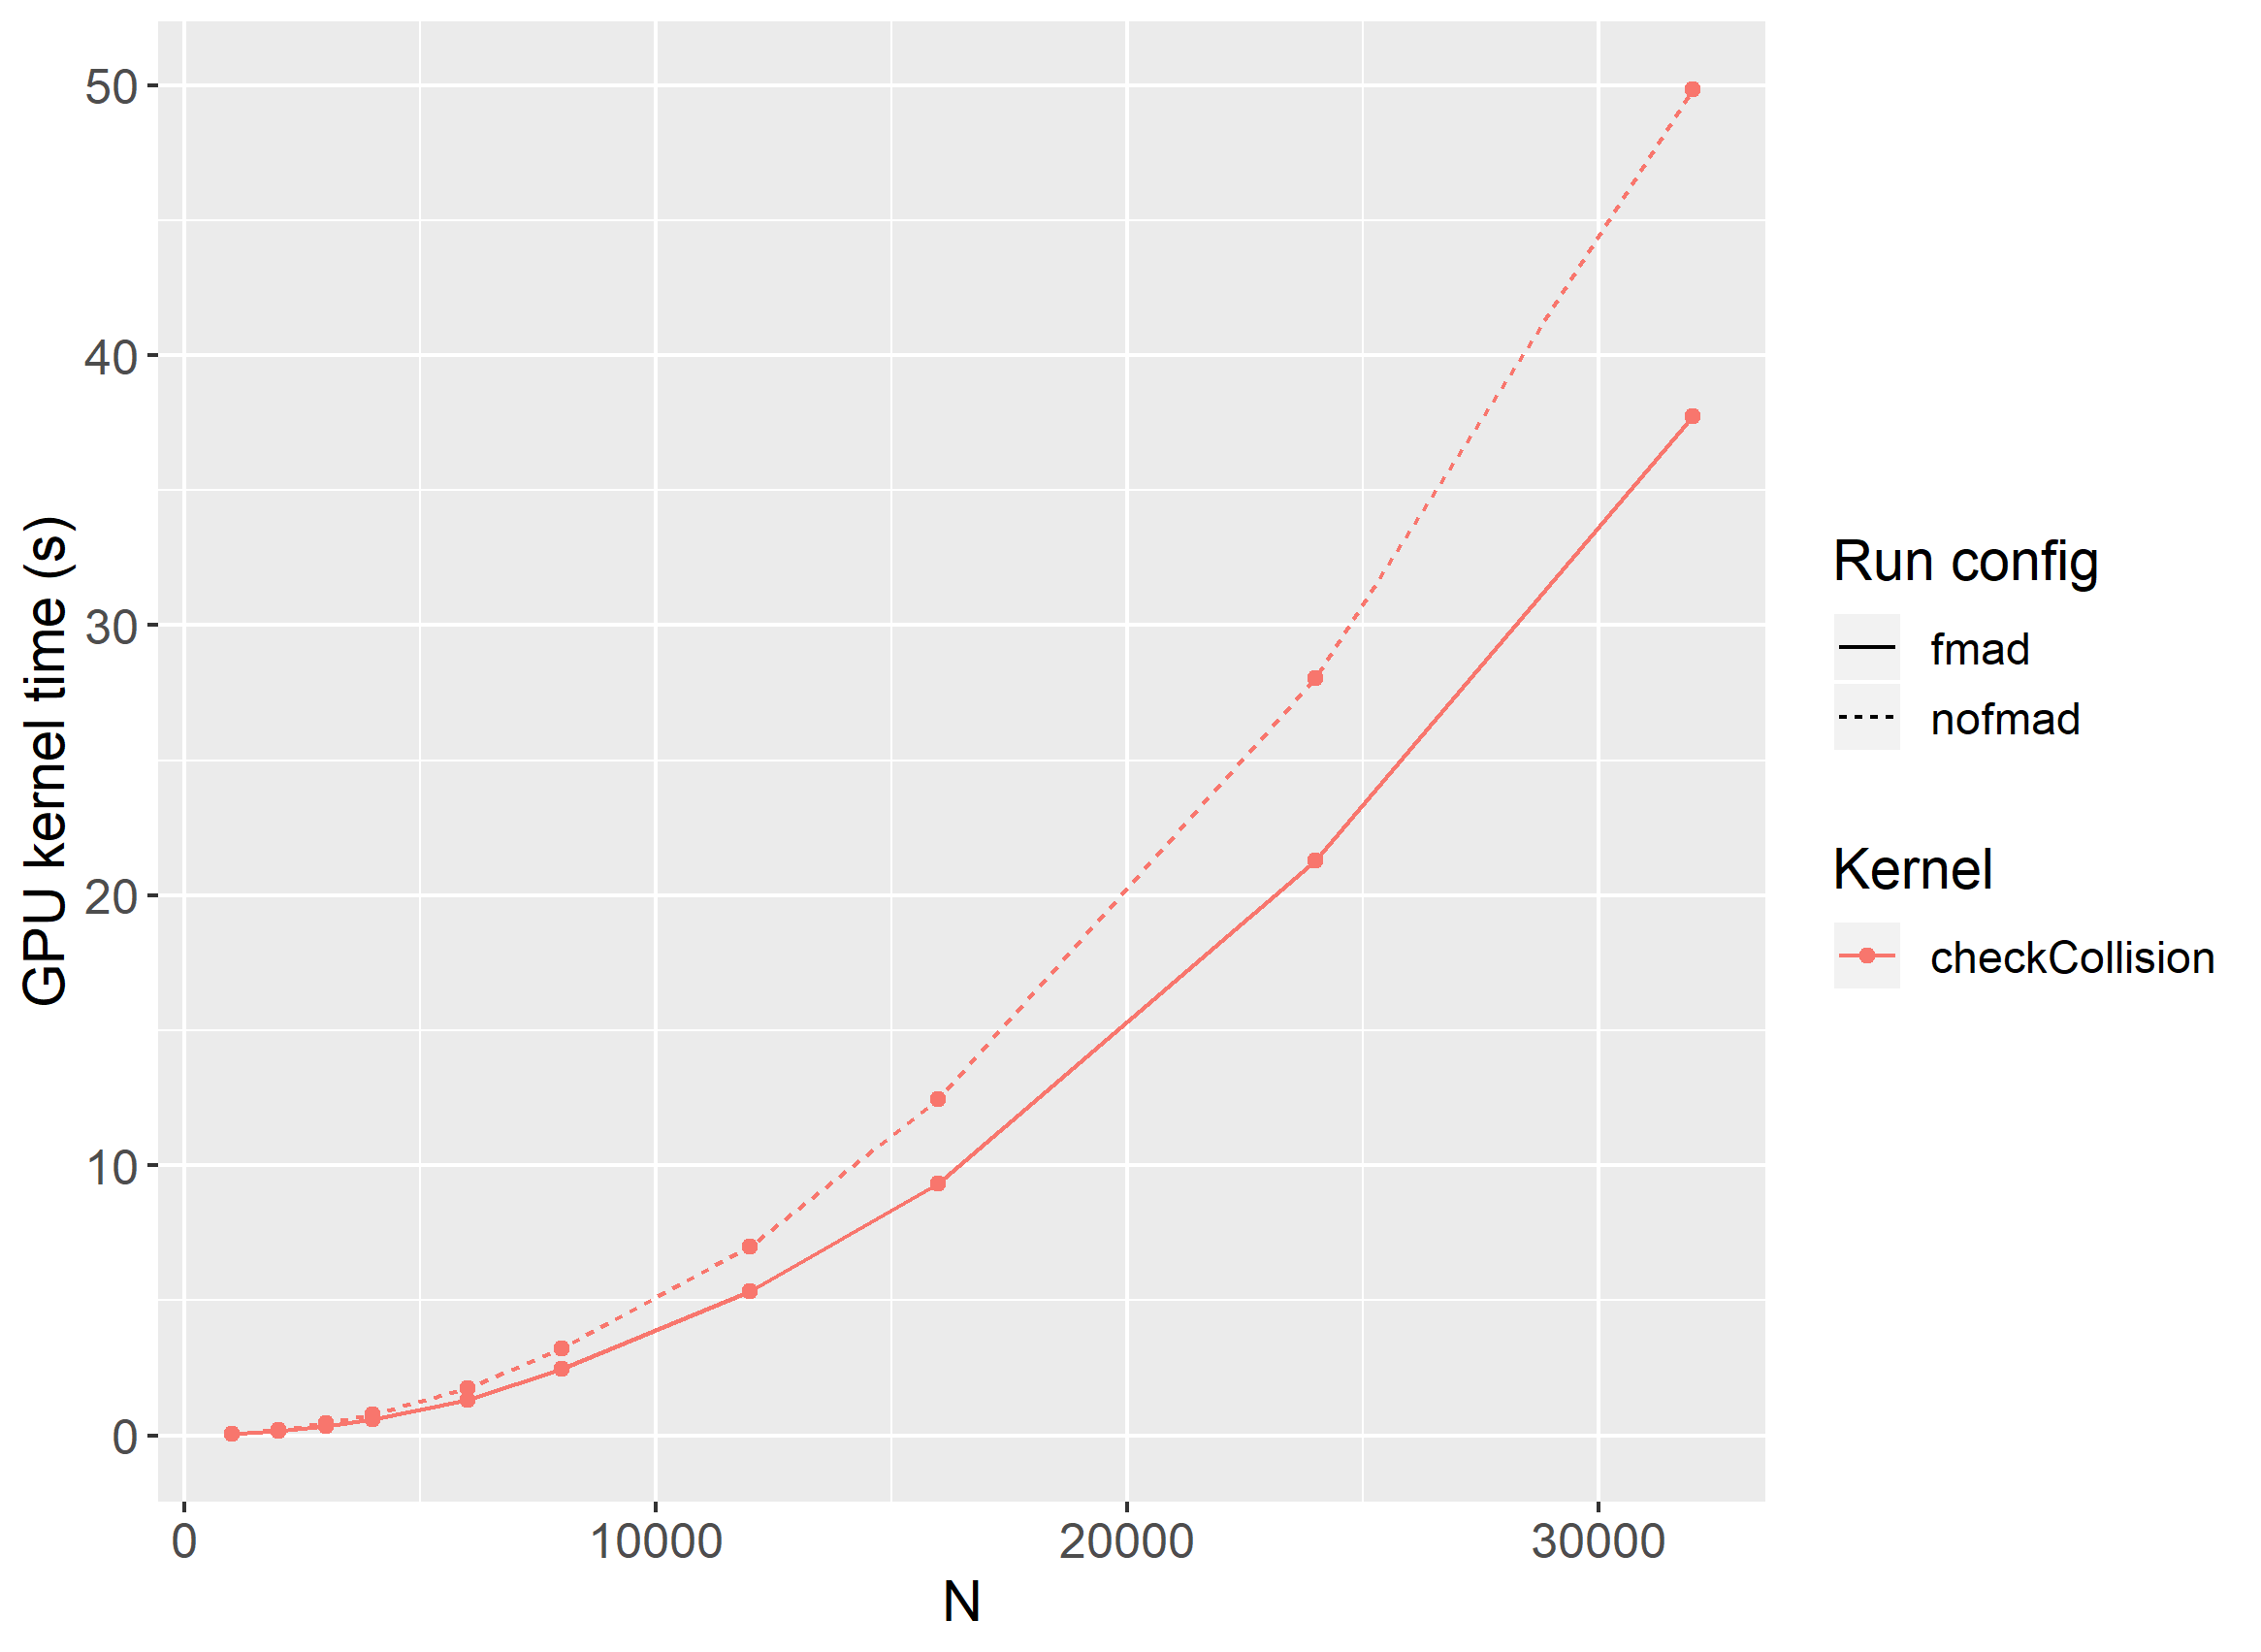
\includegraphics[width=0.75\textwidth]{titan-fmad-kernelTime-checkCollision}
    \caption{Plot of kernel time against $N$ (only \texttt{checkCollision})}
    \label{fig:titan-fmad-kernelTime-checkCollision}
\end{figure}

\begin{figure}[H]
    \centering
    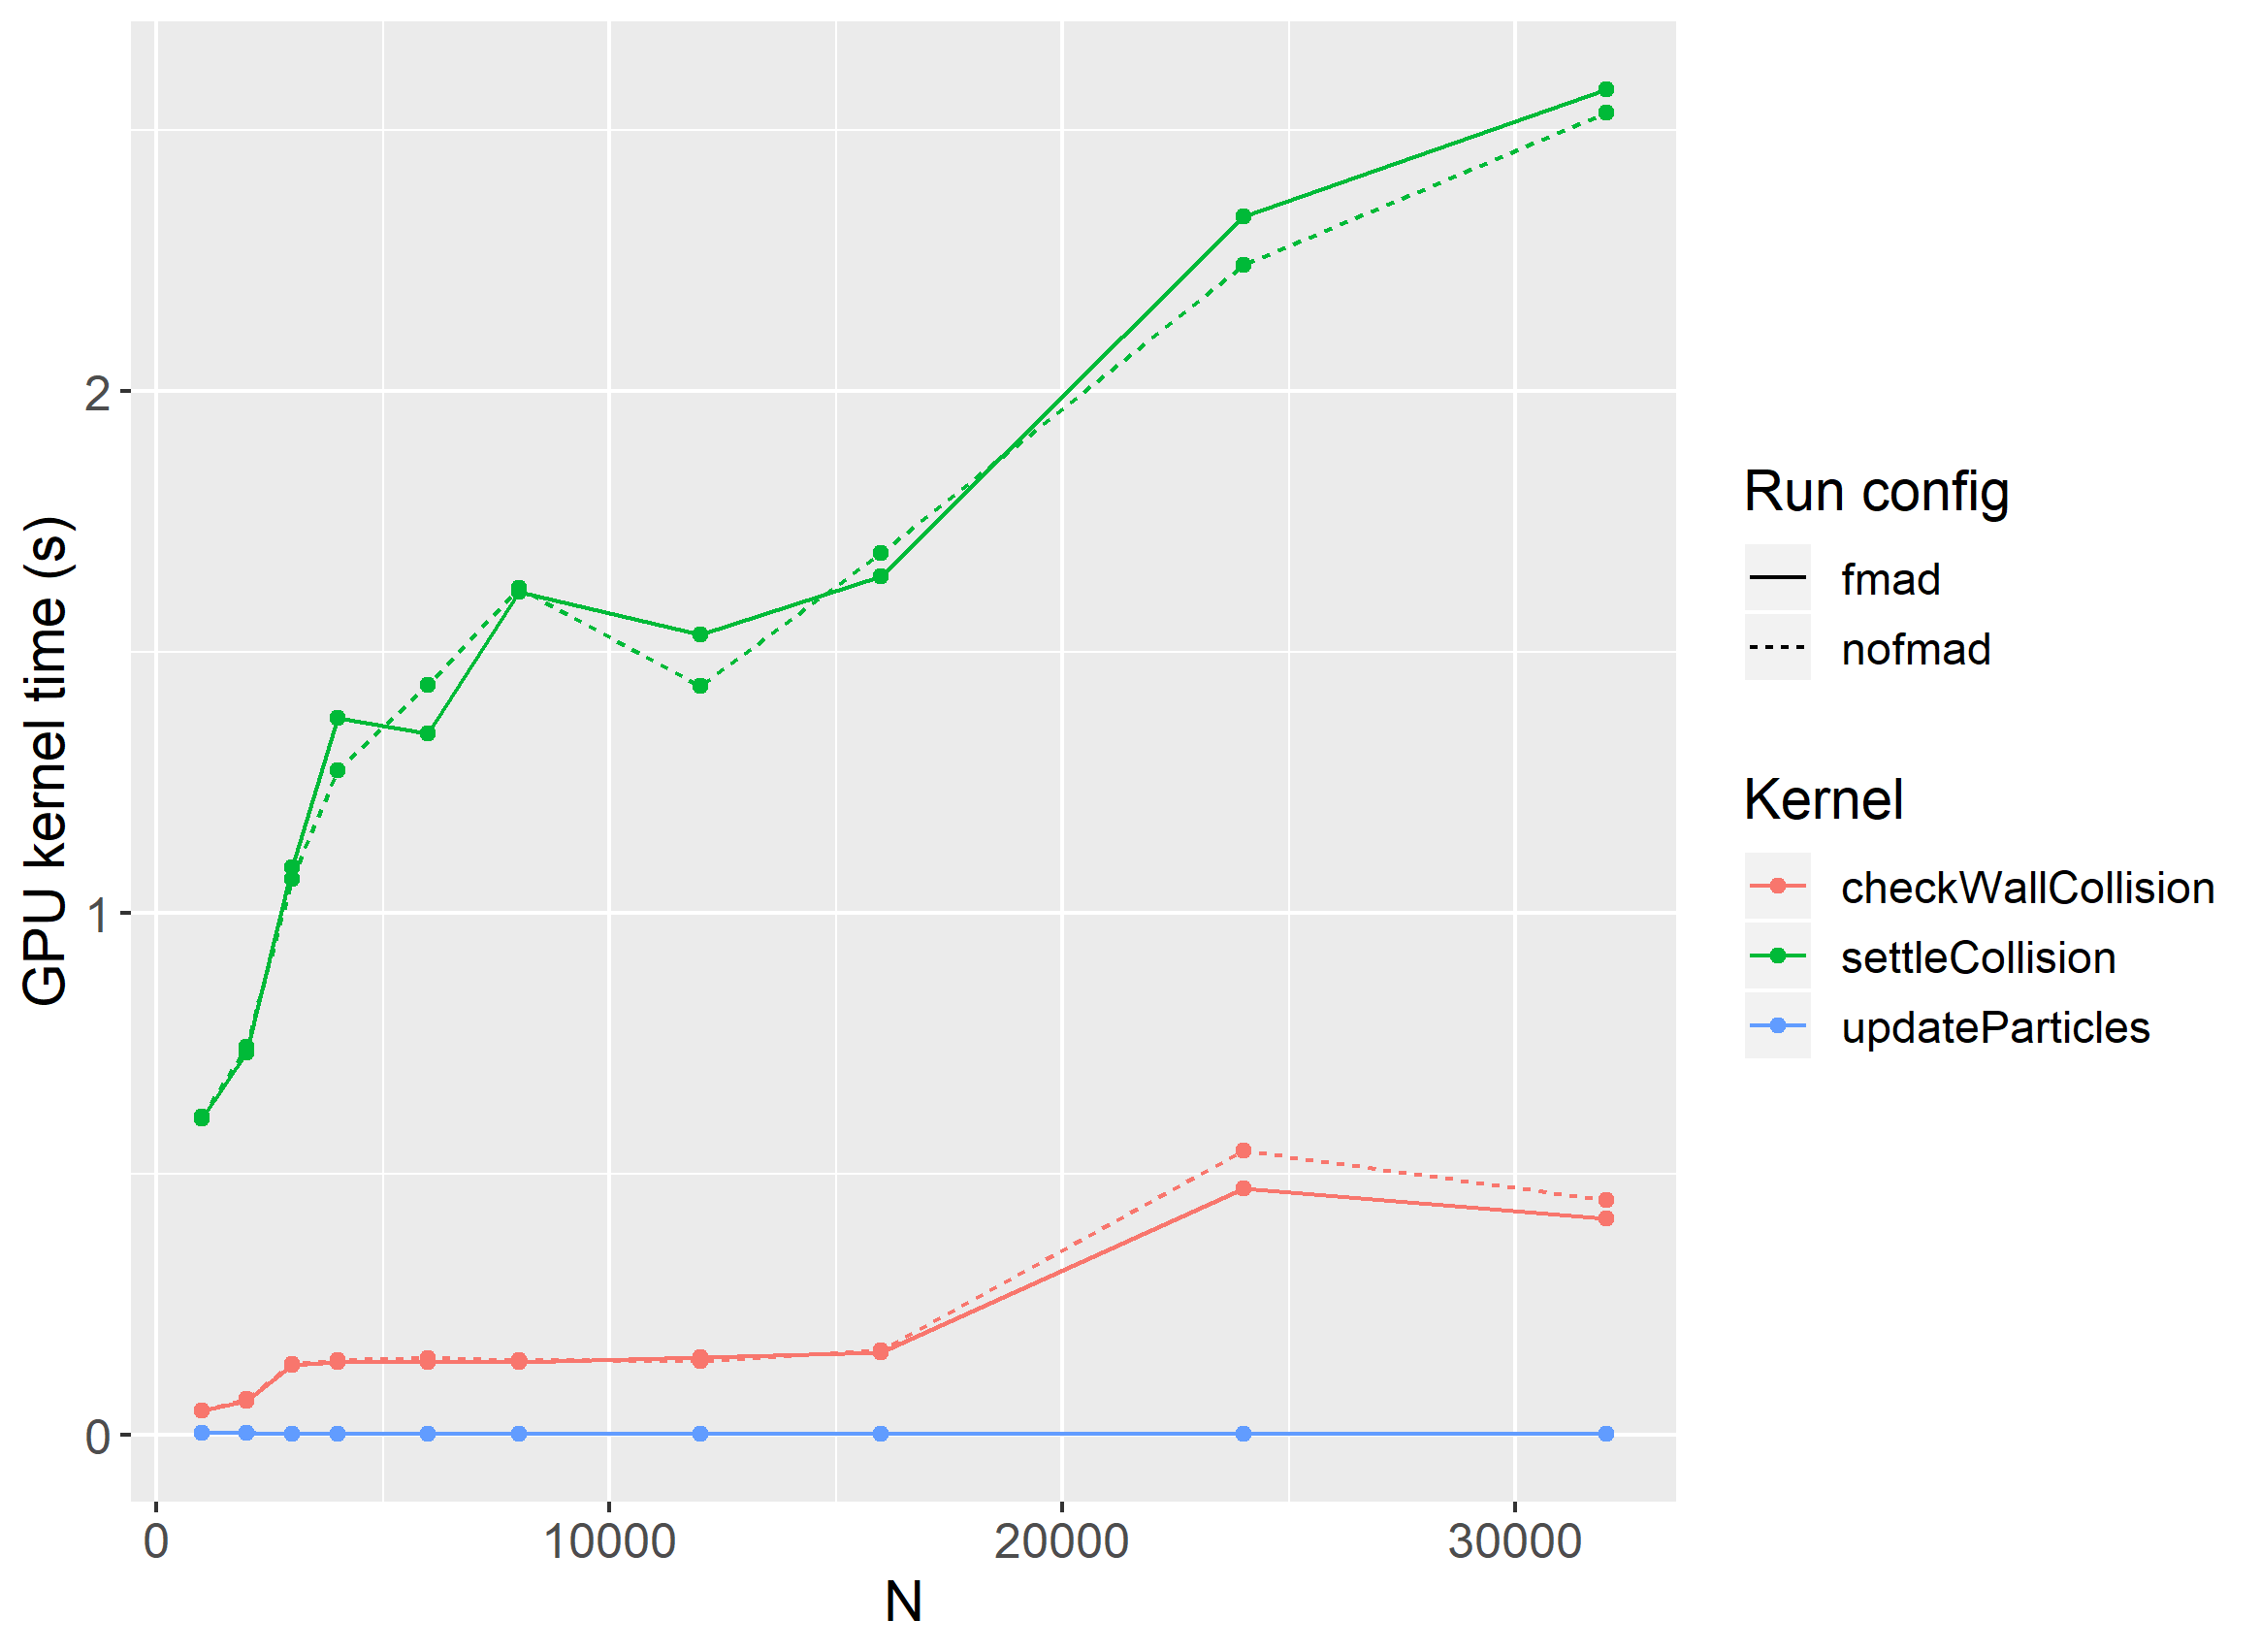
\includegraphics[width=0.75\textwidth]{titan-fmad-kernelTime-noCheckCollision}
    \caption{Plot of kernel time against $N$ (all other kernels)}
    \label{fig:titan-fmad-kernelTime-noCheckCollision}
\end{figure}

\begin{figure}[H]
    \centering
    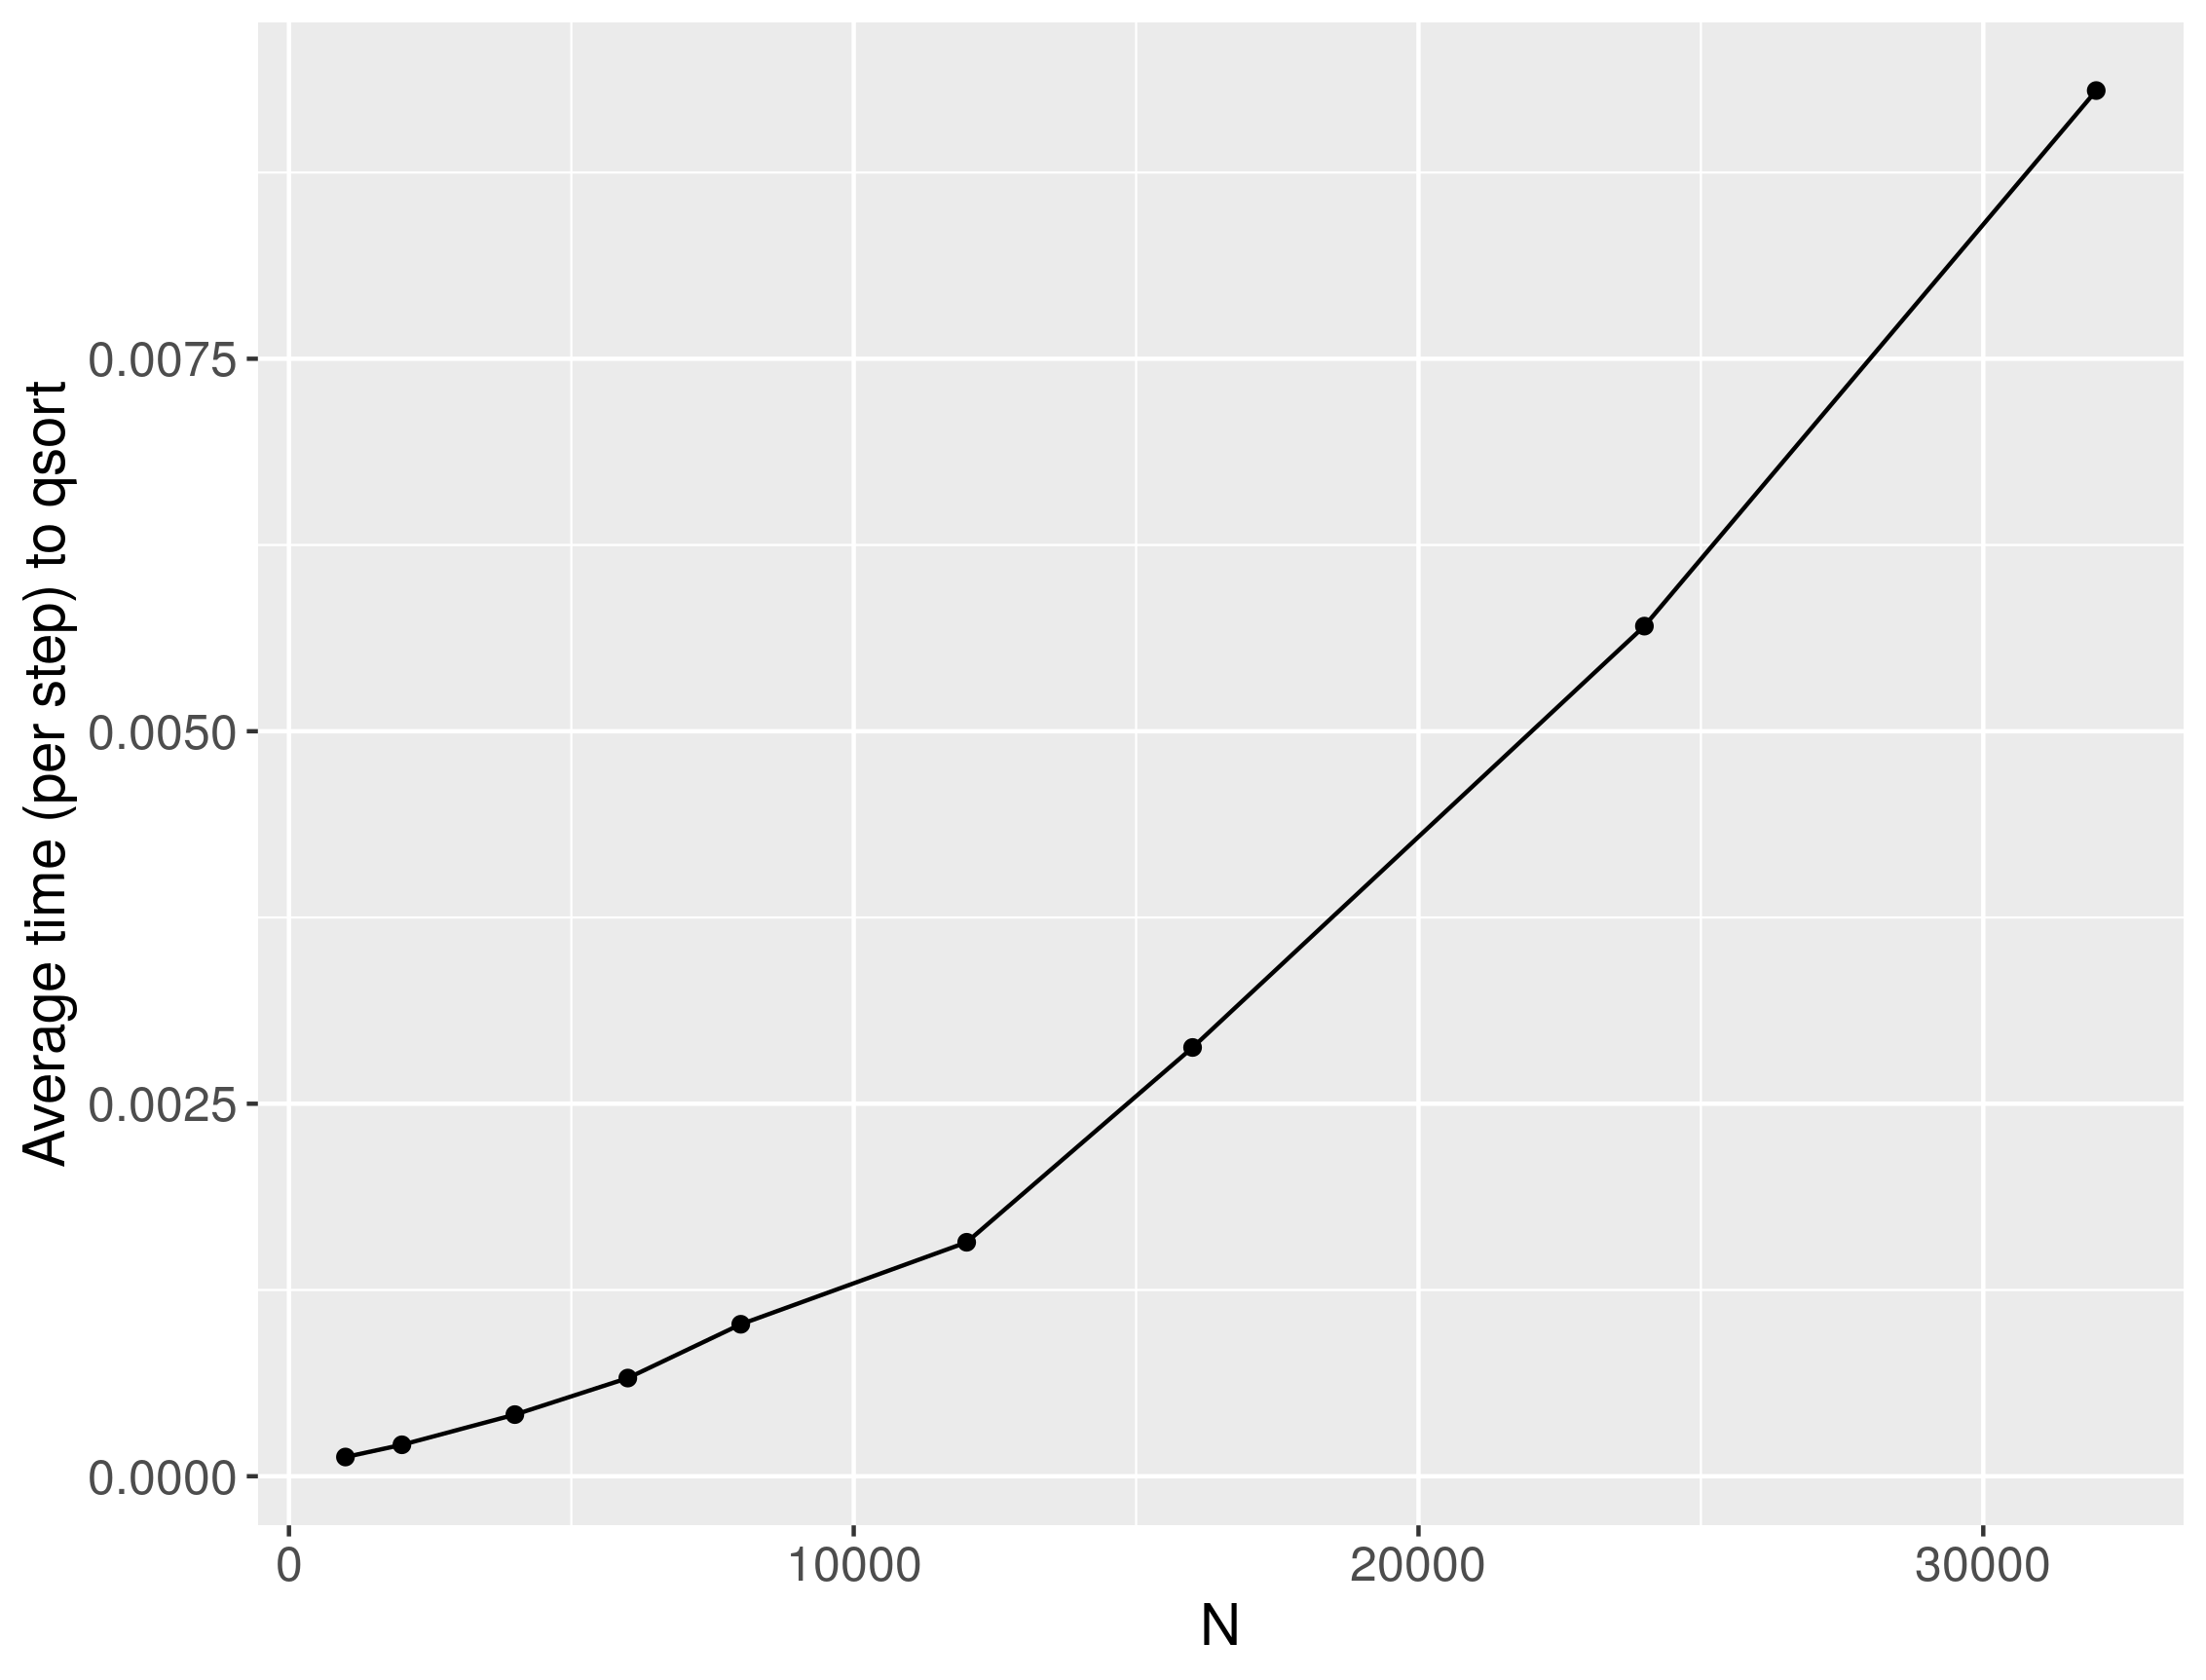
\includegraphics[width=0.75\textwidth]{avgSortTime}
    \caption{Plot of average time of \texttt{qsort} and filtering per step against $N$}
    \label{fig:avgSortTime}
\end{figure}

\pagebreak

\section{Discussion: CUDA Implementation}

\subsection{Expectations}
We did not expect our CUDA implementation to perform significantly better than the OpenMP implementation, due to the large degree of warp divergence from the many conditional statements required in a discrete particle simulator. In theory, such a computation should be very inefficient on the GPU since divergent branches are executed serially by threads in a warp.

\subsection{Observations and Comparison with OpenMP Implementation}

From Figure \ref{fig:gpu-varyN-withJetson}, we see that the execution time of the CUDA implementation maintains the same $\Theta(N^2)$ order-of-growth as the OpenMP implementation, for all GPUs and run configurations. This is expected, since we expect the runtime to be dominated by the cost of checking $\Theta(N^2)$ particle-particle collision pairs.\\

Figure \ref{fig:gpu-speedup} shows that the CUDA implementation still exhibits a significant speedup over the OpenMP implementation with 20 threads. We observe that the speedup initially grows linearly with $N$ up to some value $N_{crit}$, beyond which it quickly tapers off and displays a logarithmic nature beyond that. This is true for both run configurations, and is a clear demonstration of the rapid diminishing returns predicted by \textit{Amdahl's law}. Additionally, $N_{crit}$ was larger for the Titan RTX, which is expected as the Titan RTX has 72 SMs (4608 CUDA cores) as oppposed to the 40 SMs (2560 CUDA cores) of the Tesla T4.\\

Comparing run configurations (value of the \texttt{fmad} compiler flag), Figures \ref{fig:gpu-varyN} and \ref{fig:gpu-speedup} clearly demonstrate that the (default) \texttt{fmad} program also seems to outperform the non-\texttt{fmad} variant. This behaviour occurs as the merging of successive FP multiply and add instructions into FMA instructions is an optimisation employed by NVCC to improve the precision and speed of the program. See Section \ref{subsection:gpu-floating-point} for more details on precision. FMA instructions coalesce a FP multiply and an add instruction into a single instruction, saving clock cycles in the process. \\

Analysing the time taken by each kernel in Figure \ref{fig:titan-fmad-kernelTime-all}, we see that the \texttt{checkCollision} kernel exhibits the expected $\Theta(N^2)$ order-of-growth of runtime from having to compute $O(N^2)$ collisions. The \texttt{checkCollision} and \texttt{settleCollision} kernels exhibit some growth with increasing $N$ (albeit not linearly as expected), whereas the trend for \texttt{updateParticles} was not discernible. \\

Interestingly, we note that the \texttt{--fmad} flag only had an effect on the execution time of the \texttt{checkCollision} kernel, and did not meaningfully affect the execution time of the other three kernels. We propose two reasons for this:
\begin{itemize}
    \item The quadratic order-of-growth of runtime of this kernel makes the effect of the FMA optimisation easier to observe at large $N$, and
    \item the \texttt{checkCollision} kernel is primarily computation with a smaller proportion of branching statements, relative to the other kernels.
\end{itemize}

\begin{figure}[H]
    \centering
    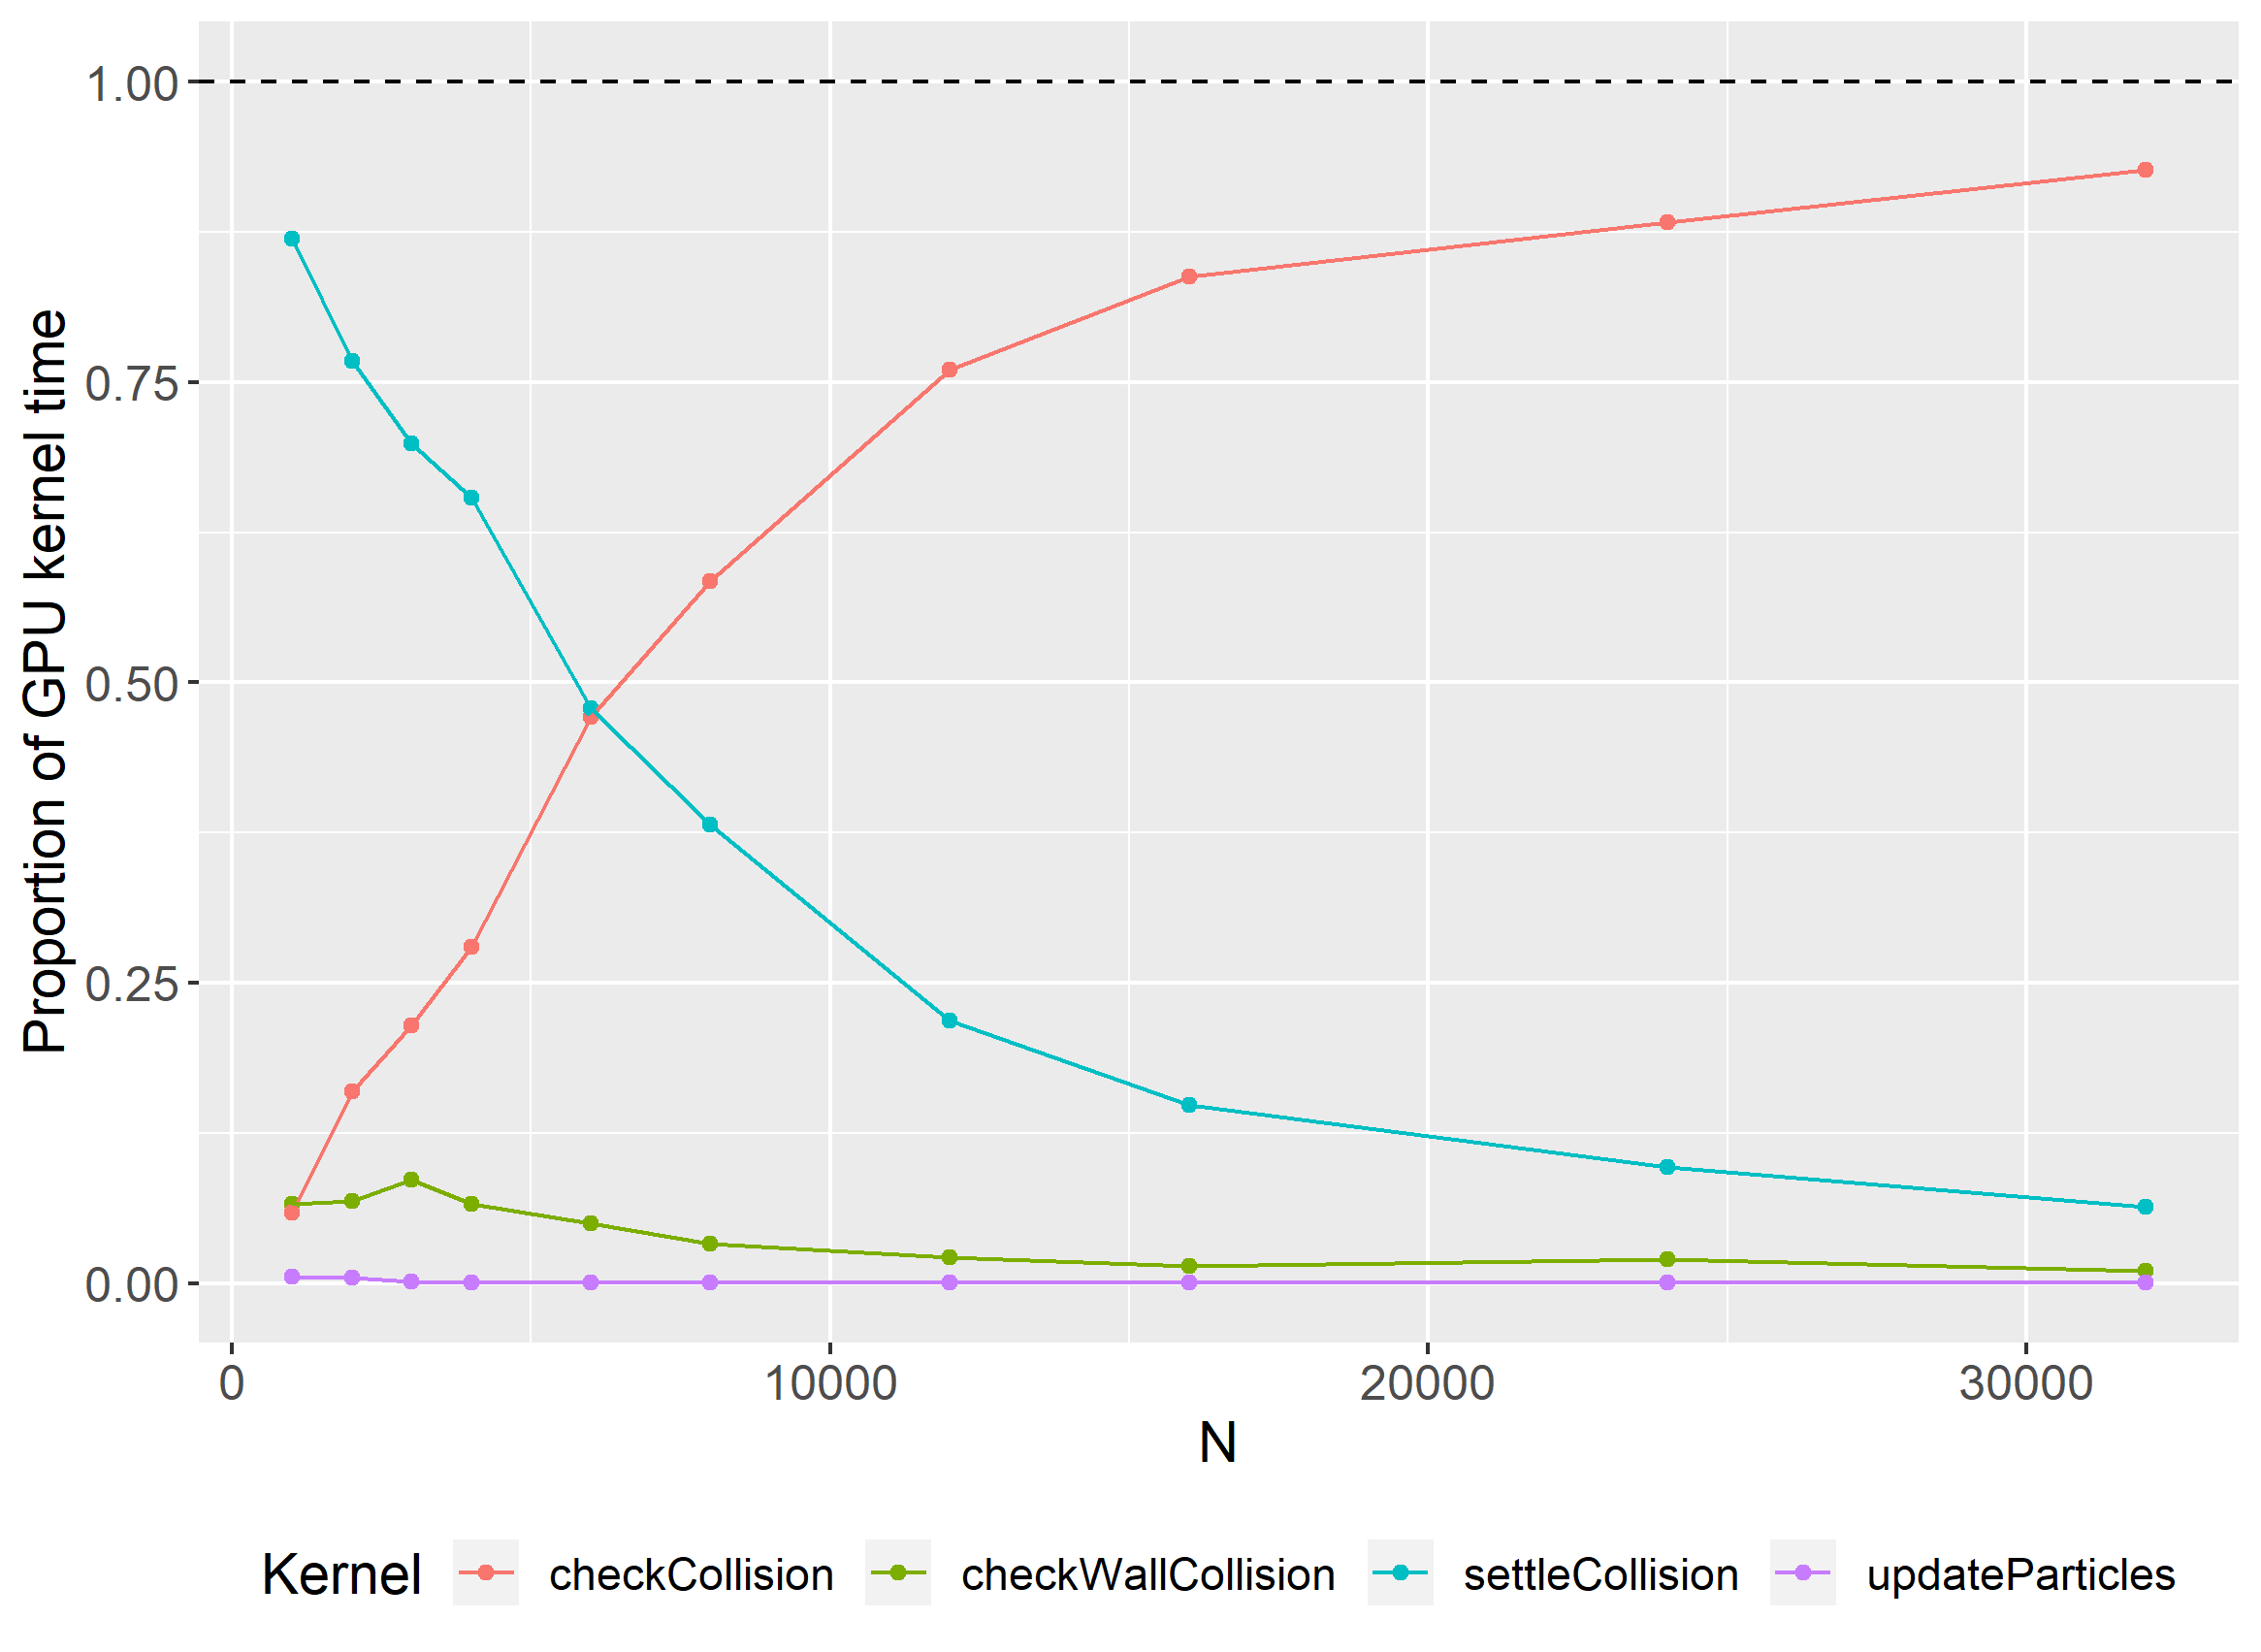
\includegraphics[width=0.75\textwidth]{titan-fmad-proportion-GPU}
    \caption{Plot of proportion of GPU runtime against $N$ for the four different kernels}
    \label{fig:titan-fmad-proportion-GPU}
\end{figure}

Comparing the fraction of total GPU time spent executing each kernel from Figure \ref{fig:titan-fmad-proportion-GPU}, we see that the \texttt{checkCollision} kernel dominates quickly with increasing $N$, in line with expectations. More interestingly, the \texttt{settleCollision} kernel dominates the overall execution time for smaller $N$, reaching parity with with \texttt{checkCollision} at about $N = 6000$ and decreasing in contribution thereafter. This behaviour is likely due to the amount of computation required to resolve a collision being larger (more conditional statements) than that required to check a potential particle-particle collision. The remaining kernels perform relatively modest work and are completed relatively quickly regardless of $N$.\\

Of particular note is the \texttt{qsort} and filtering that we did not parallelise, opting for it to be performed on the host instead. We see that the time taken to \texttt{qsort} and filter appears to grow quadratically with $N$; the impact on the entire algorithm cannot be understated. For $N = 32000$ on the Titan RTX, it took on average ~8ms for the host to complete the task - or a total of ~8s overall throughout the entire simulation, which is almost one-sixth the total execution time.\\

This behaviour can be explained. As the box size remains constant but $N$ grows, we expect the number of particle-particle collisions (of which there are $\Theta(N^2)$) to increasingly dominate over the number of particle-wall collisions (only of $\Theta(N)$), since each particle now intersects the trajectory of more particles. This is empirically confirmed by Figure \ref{fig:collisionType} below, which plots the ratio of p-p to p-w collision in the collision candidates array.

\begin{figure}[H]
    \centering
    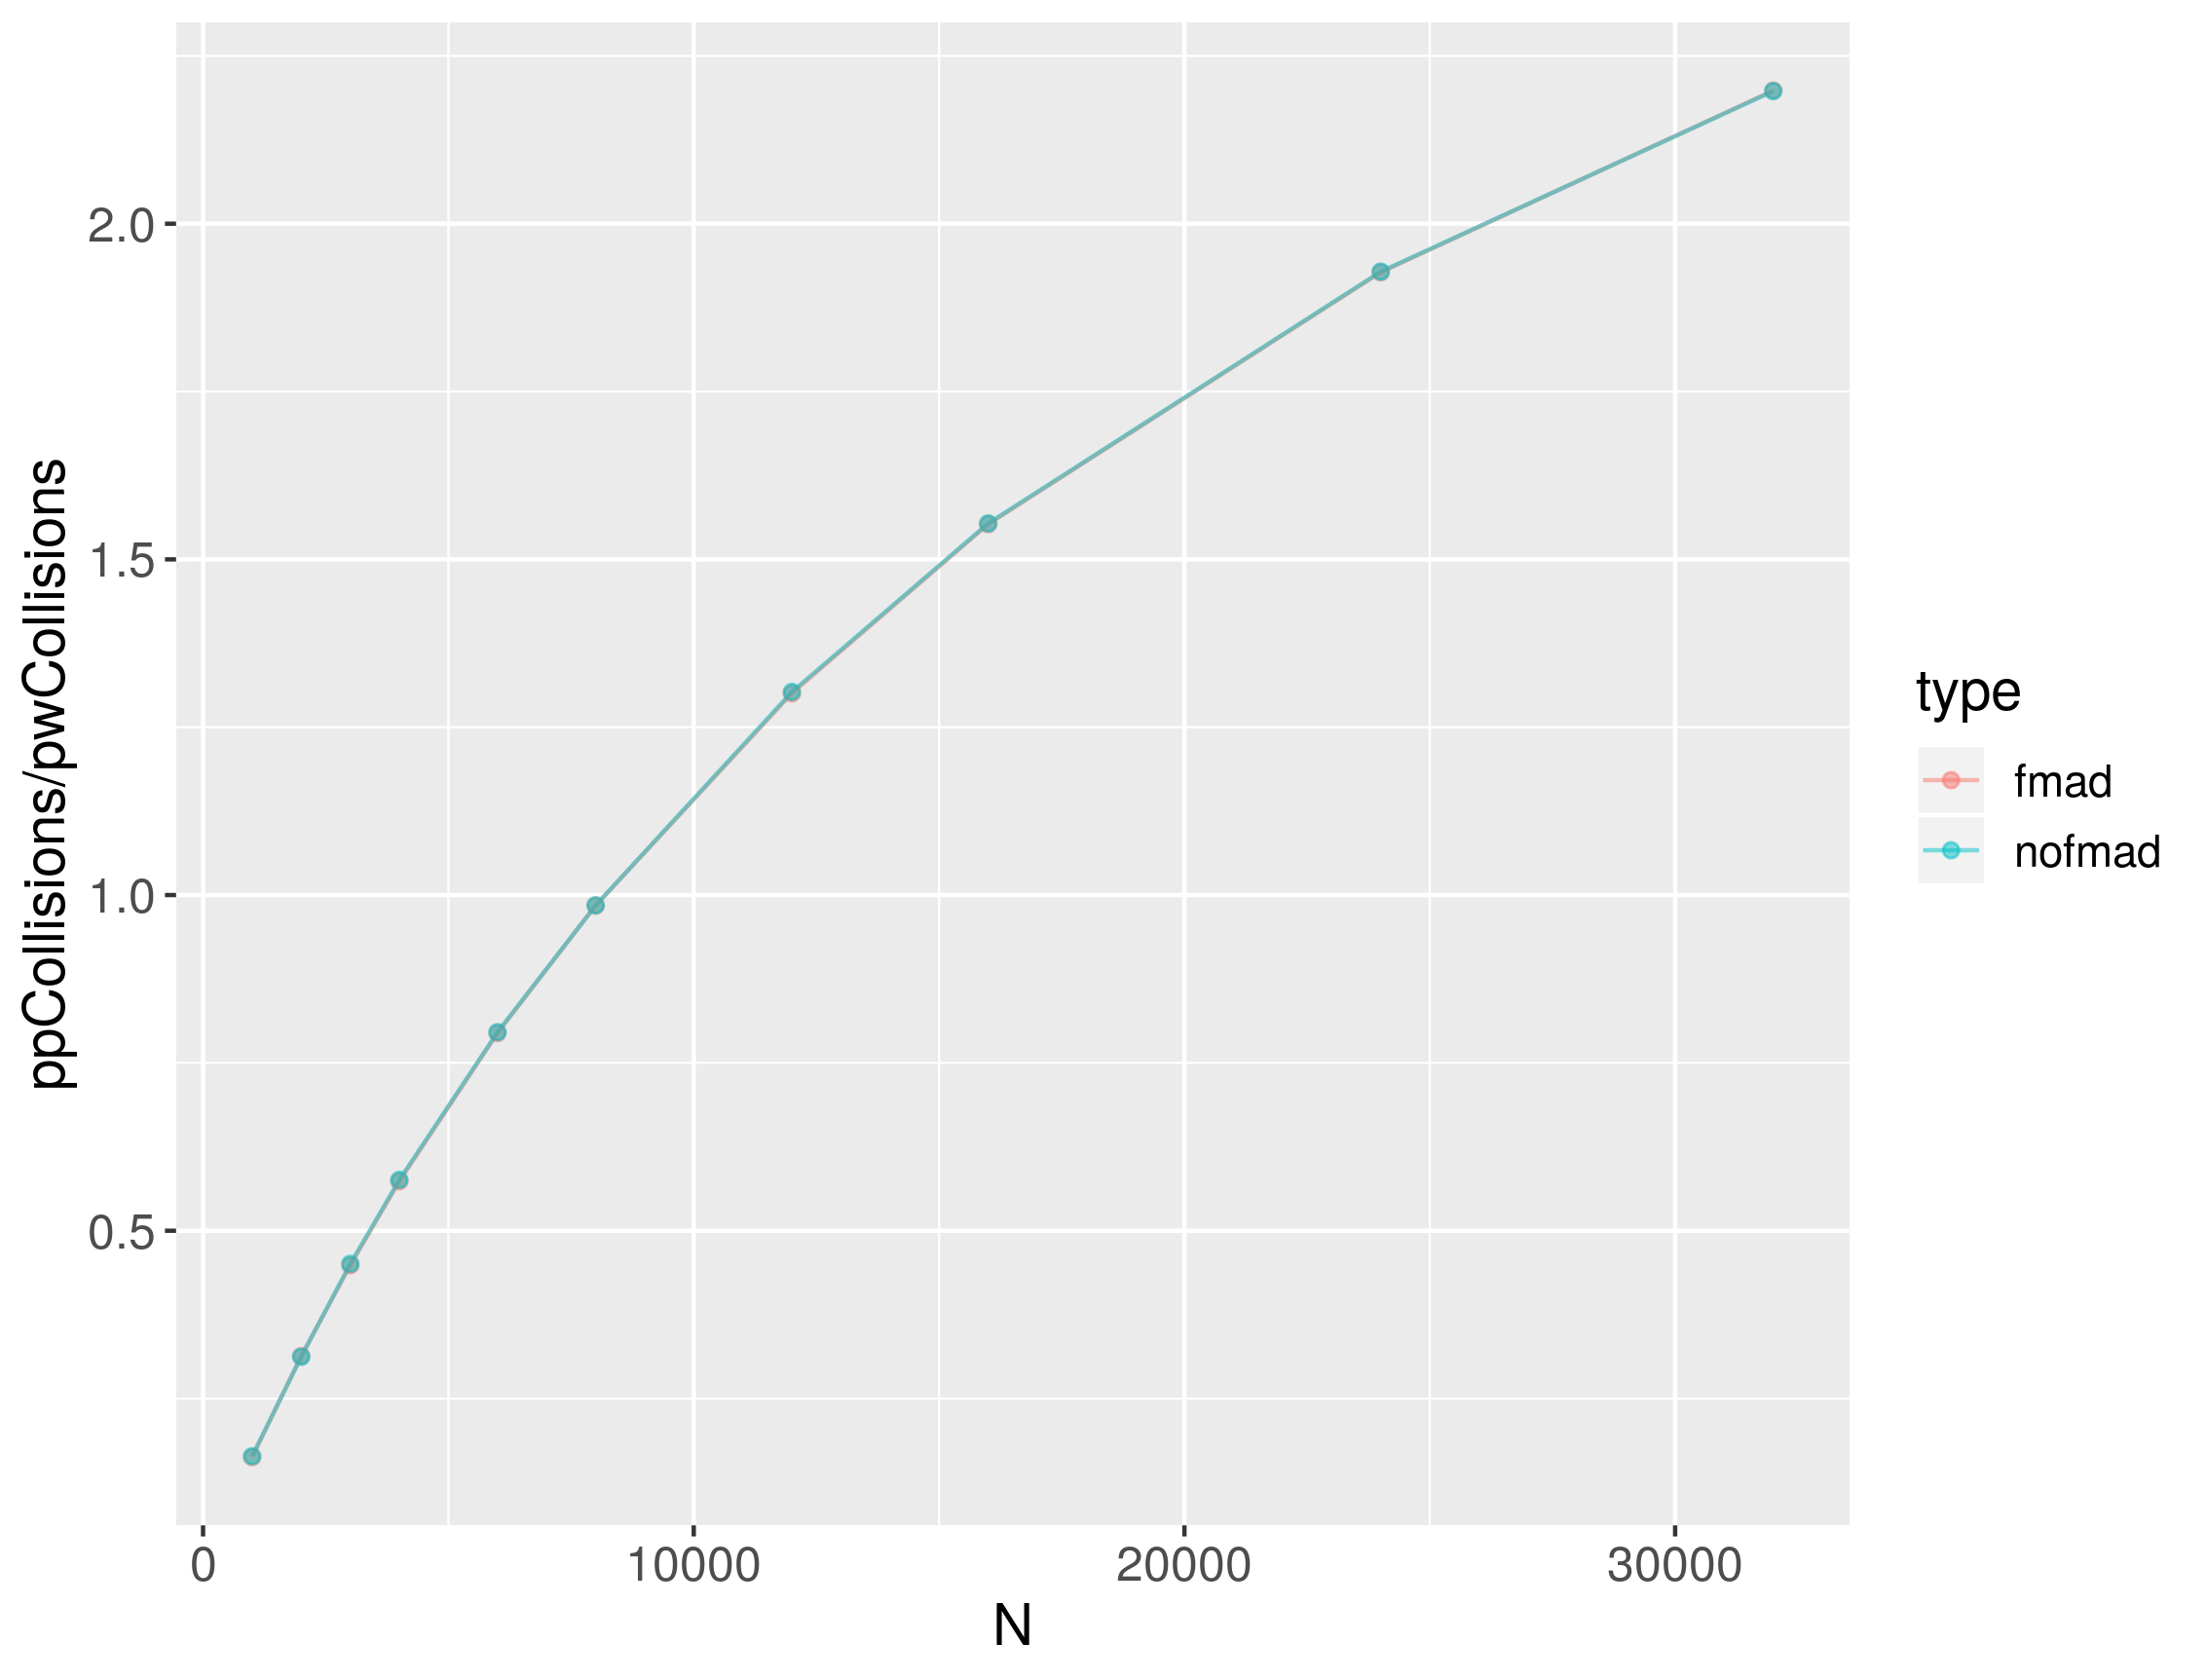
\includegraphics[width=0.75\textwidth]{collisionType}
    \caption{Plot of ratio of particle-particle collisions to particle-wall collisions against $N$}
    \label{fig:collisionType}
\end{figure}

Therefore, we expect the number of total collision candidates $N_{cand}$ to grow approximately quadratically with $N$, i.e. for large $N$, $N_{cand} \approx kN^2$. Since the runtime of quicksort is $\Theta(M lg M)$ to sort $M$ items, the final time complexity is $\Theta(N_{cand} lg N_{cand}) = \Theta(N^2lgN)$.

\subsection{GPU Comparison}

The Jetson-TX2 was computing at an extremely slow rate and the test cases past $N = 6000$ were skipped in the interest of time. While the Jetson-TX2 has an extremely unique architecture of having a shared device and host memory, it is not scalable to large problem sizes and its benefits, if any, were not demonstrated for this discrete particle simulation. \\

Considering the two main GPUs, the Titan RTX significantly outperforms the Tesla, which is consistent with the computational capability of the GPUs. The Titan RTX has a total of 4608 CUDA cores across 72 SMs as opposed to the Tesla T4's 2560 CUDA cores with only 40 SMs, for a total of 80\ more CUDA cores.\\

Coupled with the higher base and boost clocks of the Titan RTX, it can perform significantly more computations per second as compared to the Tesla T4, with the rated FP64 performance of 509.8 TFLOPS being almost twice that of the Tesla T4's 254.4 TFLOPS. This behaviour is observed in Figure \ref{fig:gpu-varyN}, where the delta between the execution time of both GPUs increases with increasing $N$, with the Titan RTX being almost twice as fast when $N = 32000$.

\pagebreak

\section{Discussion: FP32 Variant}

\subsection{Expectations}
Following words of wisdom, we attempted to ``trade precision for speed" \cite{precisionforspeed}. We expect the kernels to execute much faster given that the GPUs provided to us are optimised to perform single-precision FP32 operations (32 times more hardware FP32 than FP64 units) instead of double-precision FP64 operations. Whilst we understand that this will decrease the overall accuracy of the simulation and that the much larger magnitude of FP errors will snowball in this inherently chaotic system, it may be a viable alternative in the real world to produce an algorithm that is ``nearly there".

\subsection{Implementation and Testcases}
The source files were modified in that all occurrences of `\texttt{double}' in the source files were replaced by `\texttt{float}'. The test files remained unchanged from Section \ref{section:random-testcases}.

\subsection{Results}

\begin{figure}[H]
    \centering
    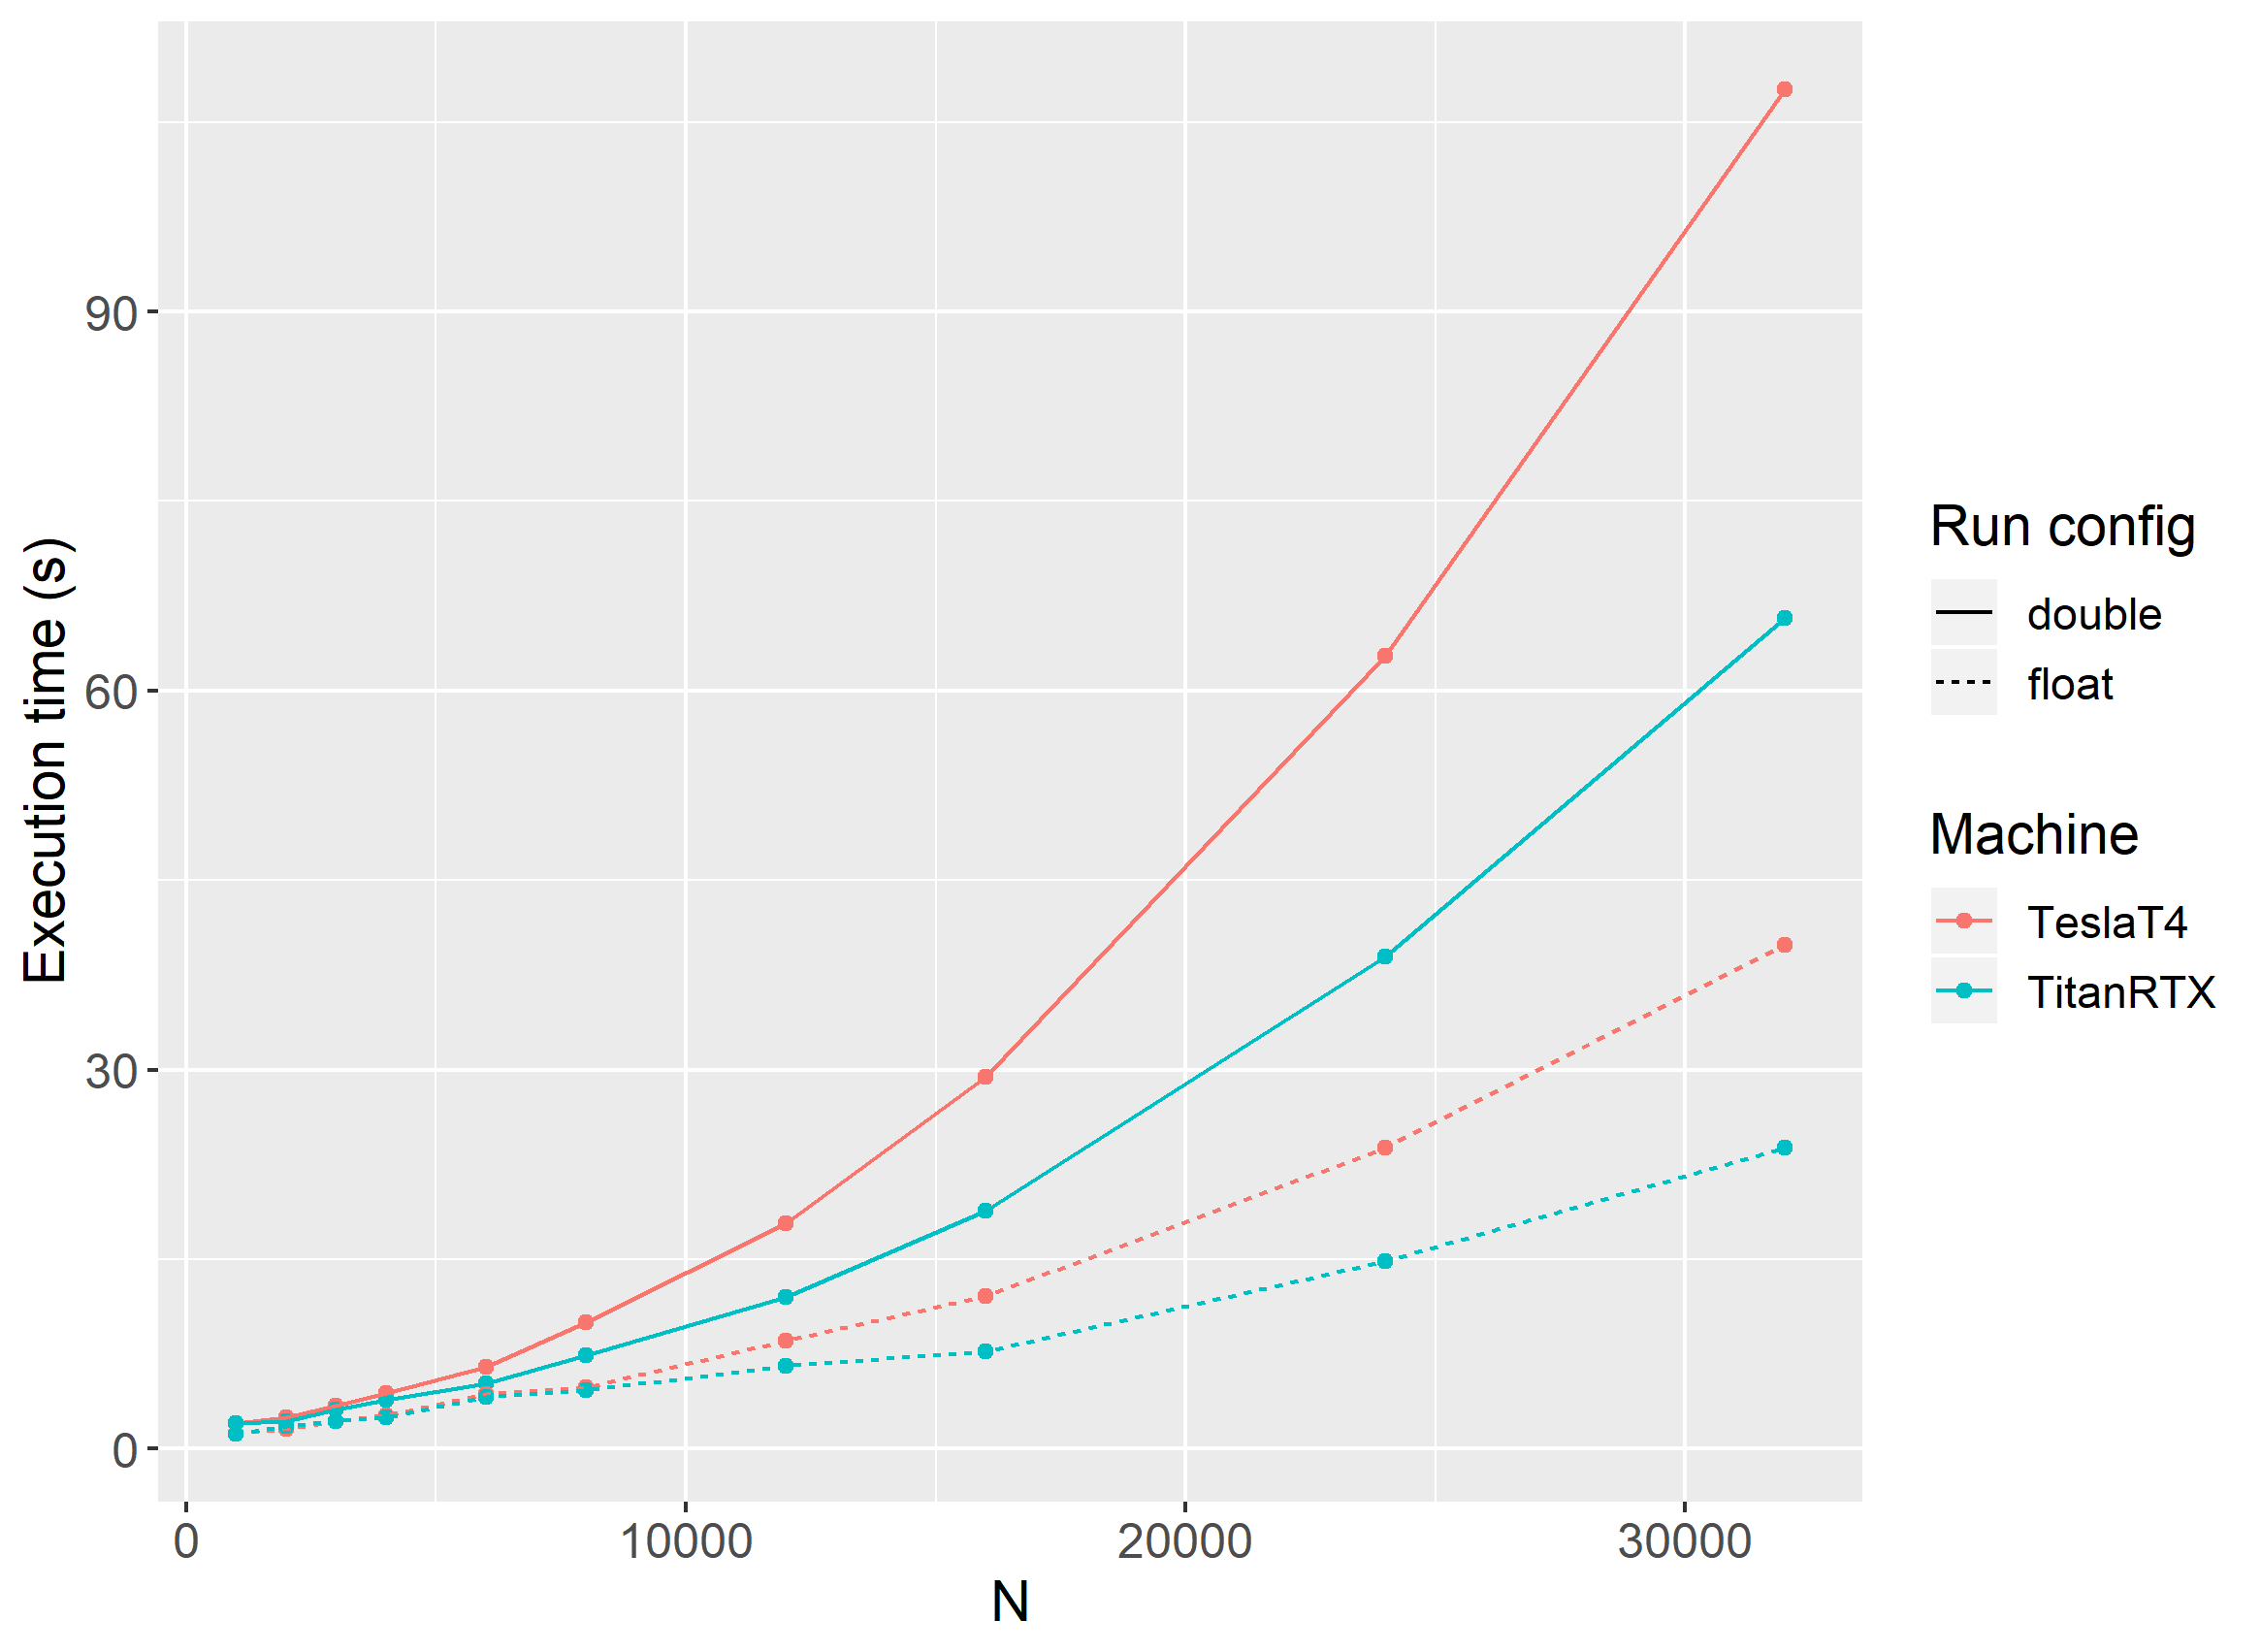
\includegraphics[width=0.75\textwidth]{double-float-comparison-fmad}
    \caption{Plot of runtime (s) against $N$ for \texttt{float} and \texttt{double} programs (\texttt{--fmad=true})}
    \label{fig:double-float-comparison-fmad}
\end{figure}

\begin{figure}[H]
    \centering
    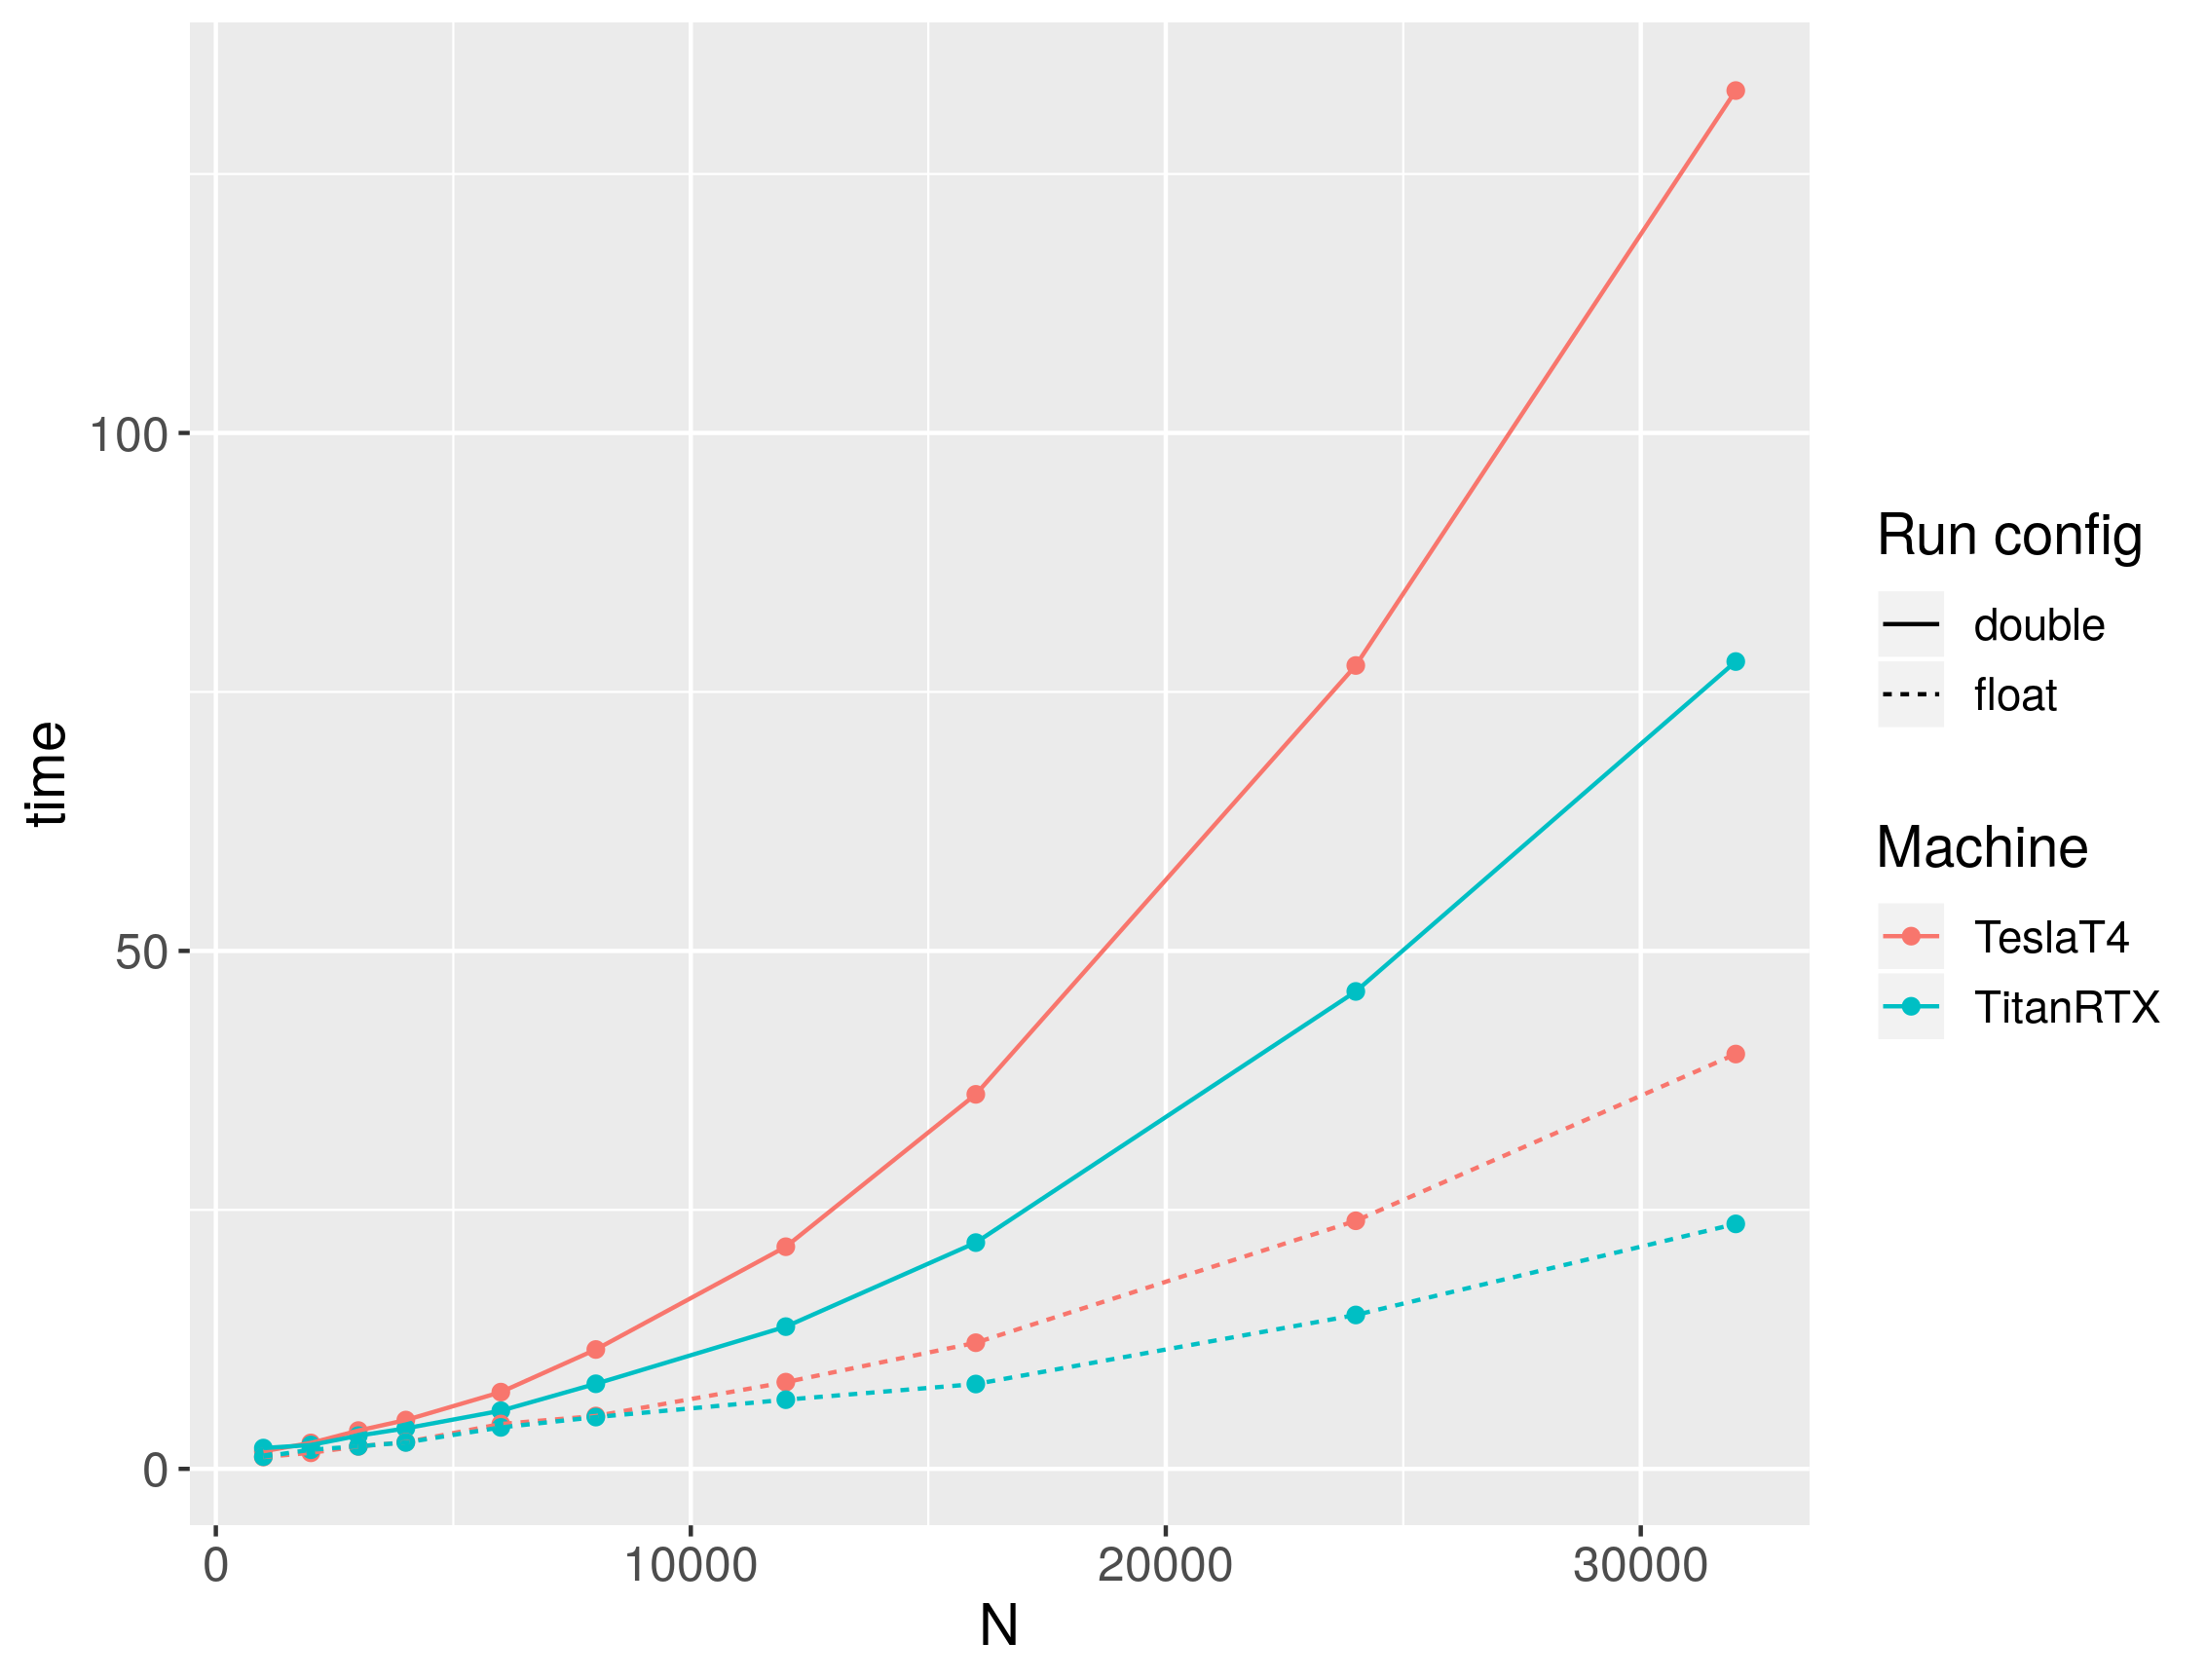
\includegraphics[width=0.75\textwidth]{double-float-comparison-nofmad}
    \caption{Plot of runtime (s) against $N$ for \texttt{float} and \texttt{double} programs (\texttt{--fmad=false})}
    \label{fig:double-float-comparison-nofmad}
\end{figure}

While it is clear that the implementation using \texttt{float}s outperformed the one using \texttt{double}s, the measured speedup fails to reach the factor of 32 that we had expected (from comparing the rated FP32 to FP64 throughput in TFLOPS).\\

Instead, the change only resulted in a speedup of between $2-3$. We propose two reasons for this deviation:
\begin{itemize}
    \item The overhead from synchronisation required to add new collision candidates becomes significant for large $N$, since many more threads are attempting to increment the global counter \texttt{numCollisions} with \texttt{atomicAdd}
    \begin{itemize}
        \item Multiple threads (within and across warps) contending to perform the same operation on a single memory address leads to serialisation of the operations, exacerbating the delay of atomic operations
    \end{itemize}
    \item The GPU memory subsystem may become a bottleneck for FP32 computations since we opted to use managed memory - most of the data (particle states and collision candidates) resides in the GPU's global memory, which is slow to access and becomes increasingly poorly cached as $N$ increases
\end{itemize}

\pagebreak

\section{Discussion: Chunk-size Variants}

We also tried varying the chunk sizes (number of threads in each block) of the various different kernels in the program. We varied the parameters separately for the 1D kernels (\texttt{checkWallCollision}, \texttt{settleCollision} and \texttt{updateParticles}) and the 2D kernels (\texttt{checkCollision}).

\subsection{Testcases}
The simulation parameters of the modified default testcase are
\begin{itemize}
    \item Machine: Titan RTX (\texttt{xgpe1})
	\item $\textbf{N = 2000}, L=20000, r=1, S=1000$
\end{itemize}

\begin{enumerate}
	\item GPU implementation
	\begin{itemize}
		\item $C_1$ = chunk size (threads per block) of 1D kernels
		\item $C_2$ = chunk size (threads per block) of 2D kernels
		\item $F$ = \texttt{--fmad} compile flag
		\item Varying both $N$, $C_1$,  $C_2$ and $F$ together
		\begin{itemize}
		    \item $N = 2k, 3k, 4k, 6k, 8k, 12k, 16k, 24k, 32k$
			\item $C_1 = 32, 64, 96, 128, 192, 256$
			\item $C_2 = 32, 64, 96, 128, 192, 256$
			\item $F =$ \texttt{true, false}
		\end{itemize}
	\end{itemize}
\end{enumerate}

\pagebreak

\subsection{Results}

The varying of chunk sizes yielded mostly disappointing results, with little to no variance (within the standard error) across runs. The execution times of runs with varying $C_1$ and constants $N = 32000, C_2 = 64, F =$ \texttt{true}, as well as varying $C_2$ and constants $N = 32000, C_1 = 64, F =$ \texttt{true} are illustrated in Figures \ref{fig:chunkSize-1D-32000-fmad} and \ref{fig:chunkSize-2D-32000-fmad}.

\begin{figure}[H]
    \centering
    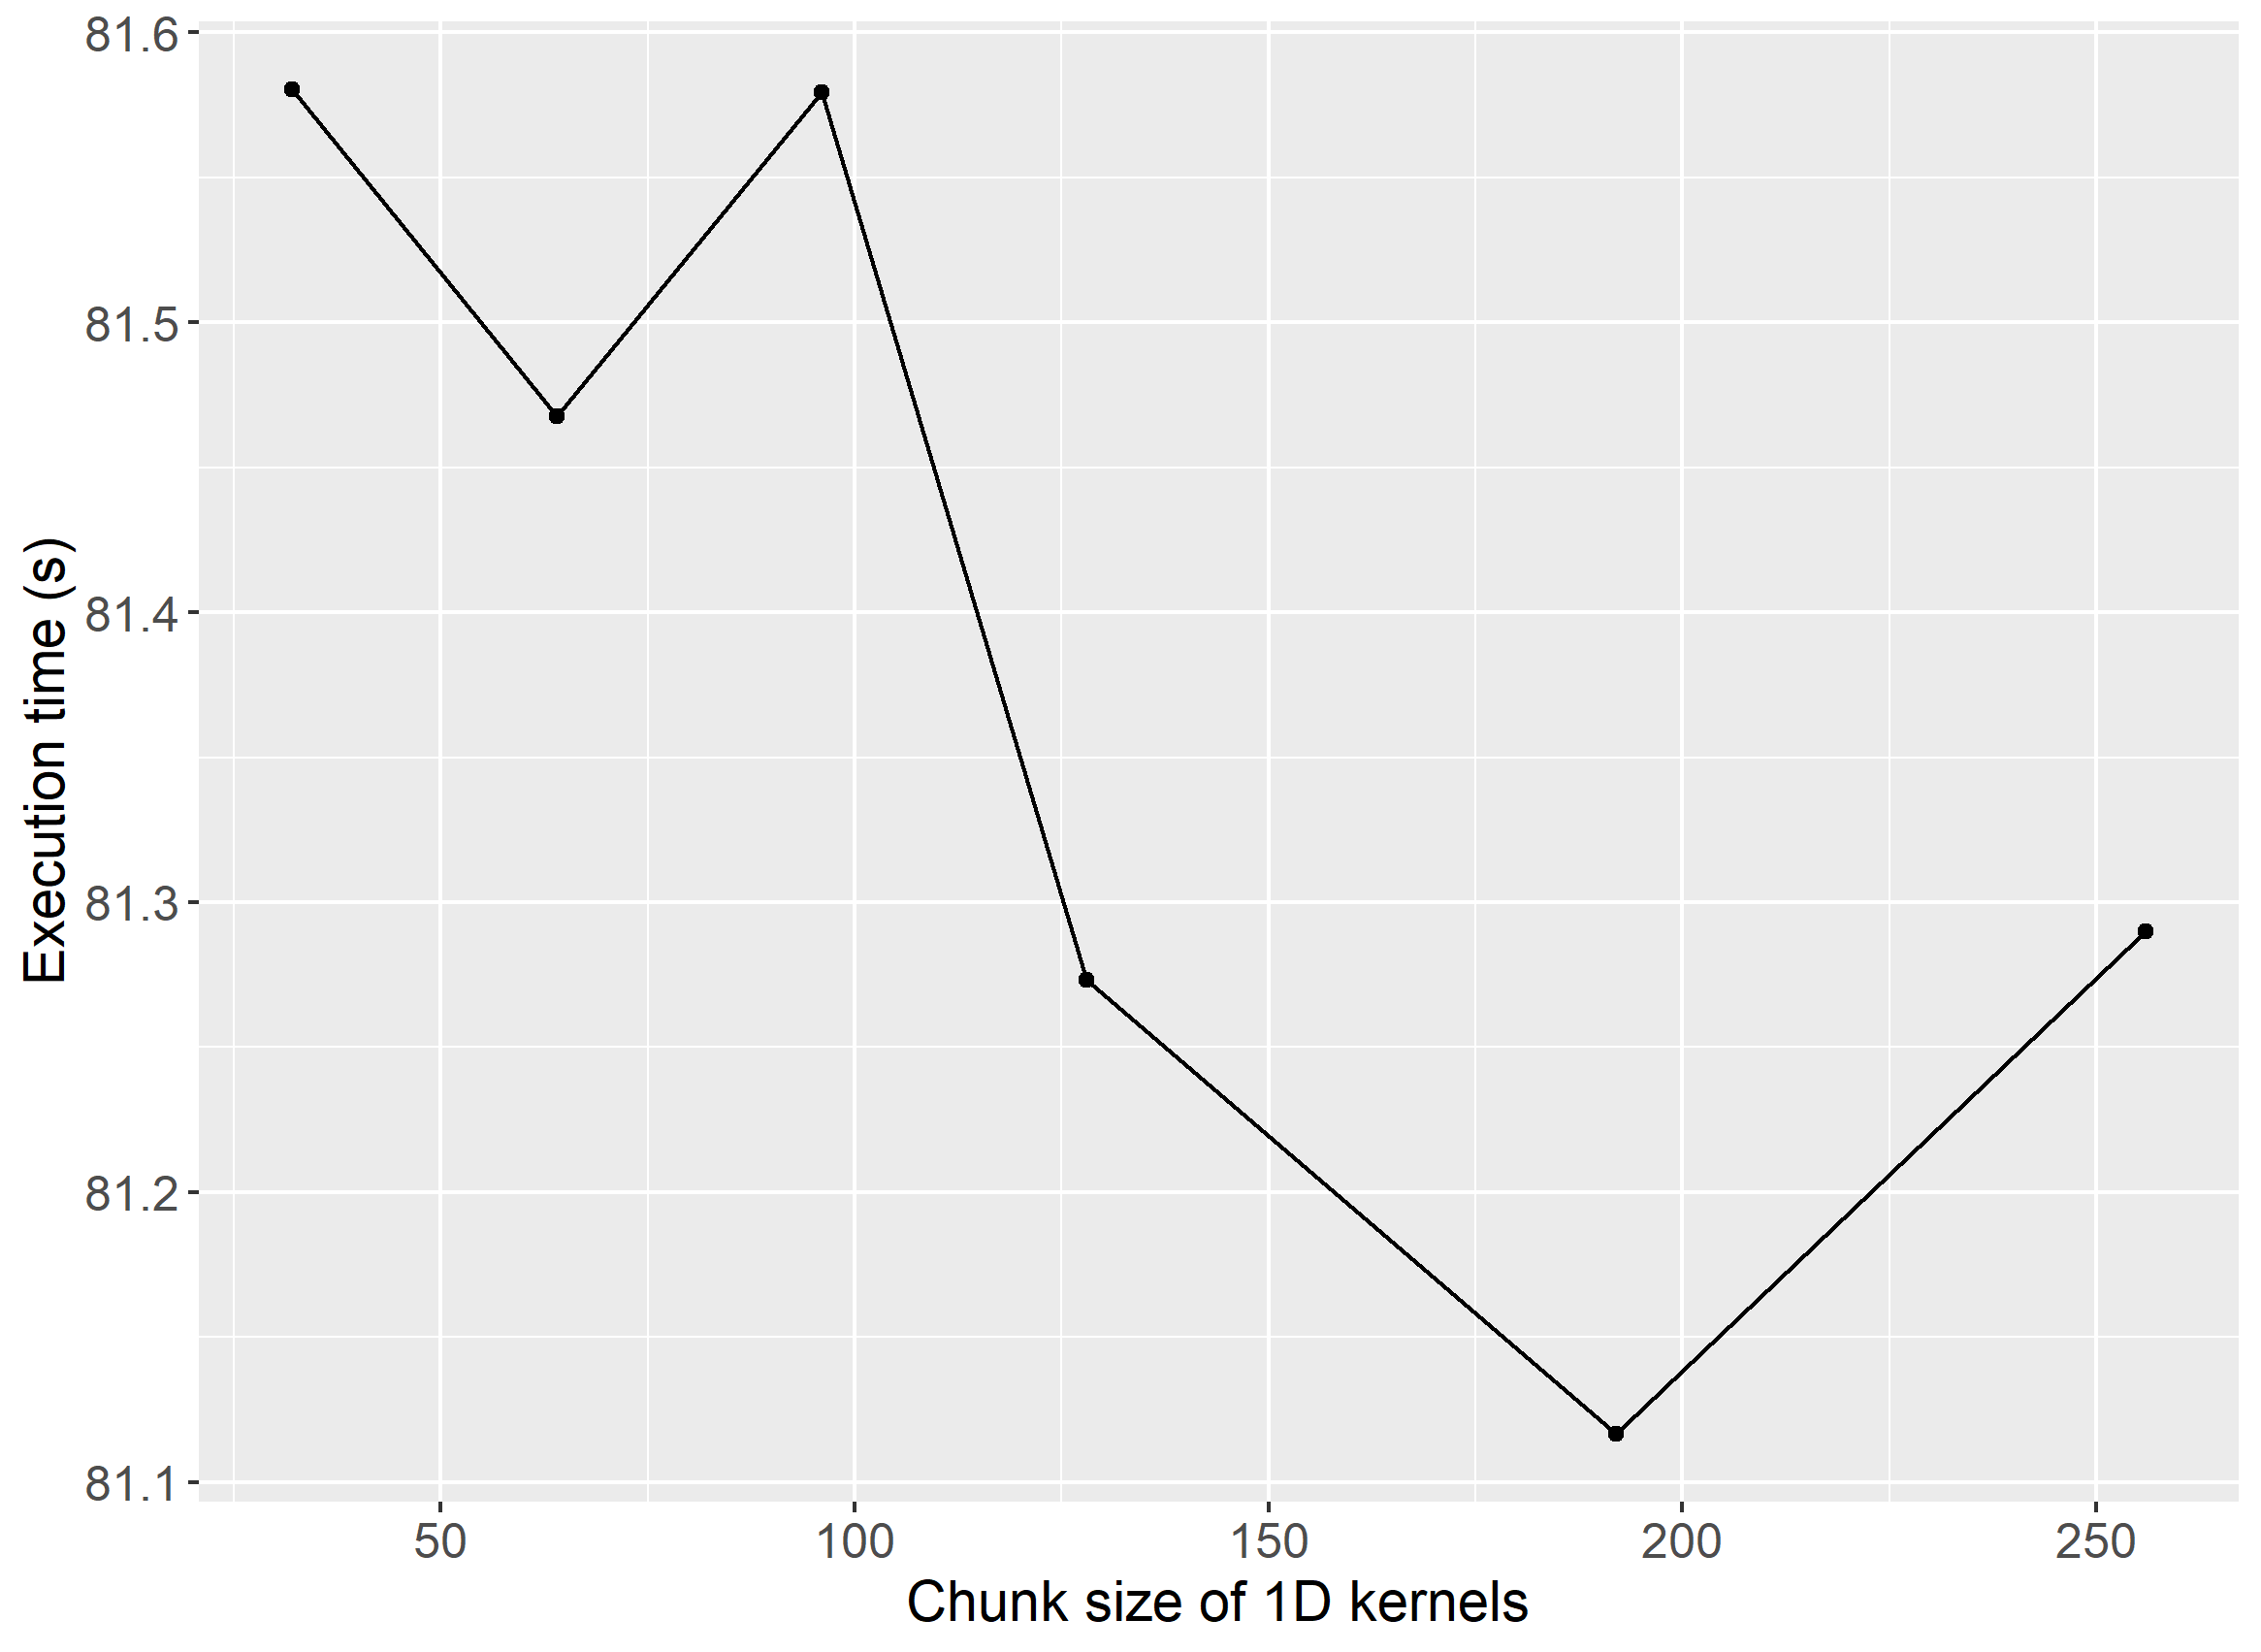
\includegraphics[width=0.75\textwidth]{chunkSize-1D-32000-fmad}
    \caption{Plot of runtime (s) against $C_1$, 1D kernel chunk size ($N = 32000, C_2 = 64, F =$ \texttt{true})}
    \label{fig:chunkSize-1D-32000-fmad}
\end{figure}

\begin{figure}[H]
    \centering
    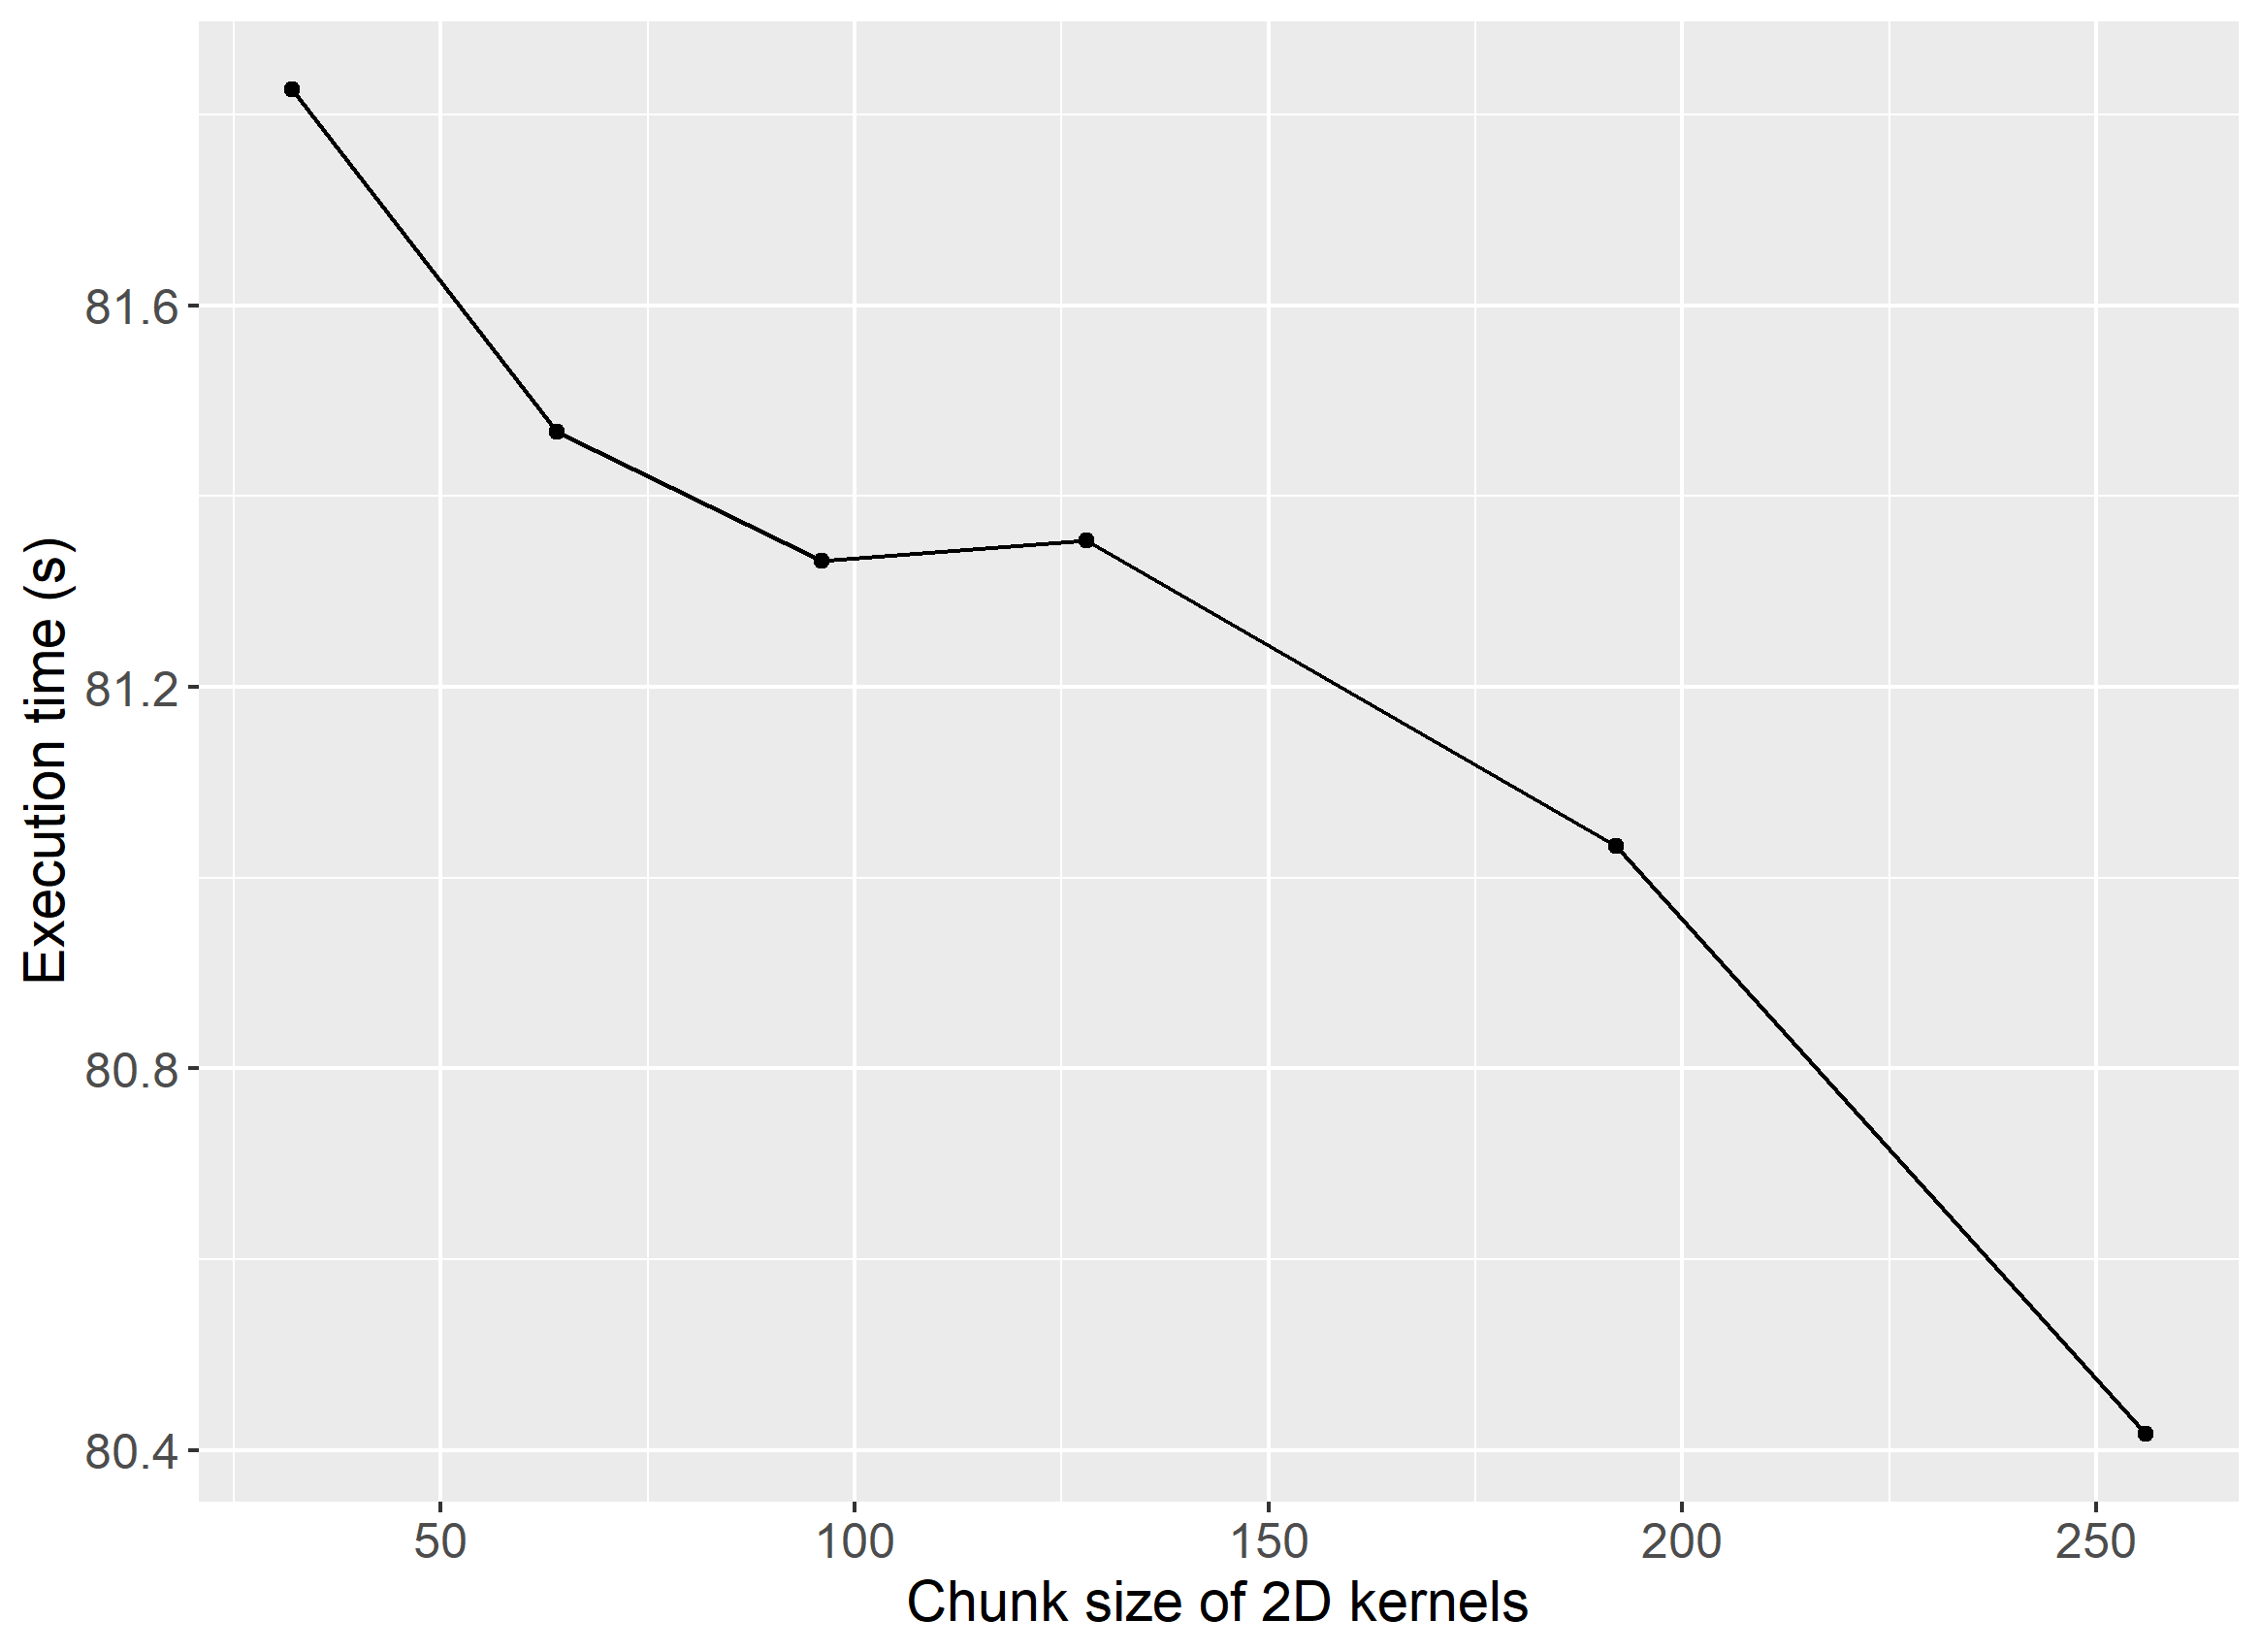
\includegraphics[width=0.75\textwidth]{chunkSize-2D-32000-fmad}
    \caption{Plot of runtime (s) against $C_2$, 2D kernel chunk size ($N = 32000, C_1 = 64, F =$ \texttt{true})}
    \label{fig:chunkSize-2D-32000-fmad}
\end{figure}

A decreasing trend is observed in runtime against increasing $C_2$ but no discernable pattern is observed for runtime against increasing $C_1$. The performance increase with increasing $C_2$, however, is very small as compared to the total runtime and we cannot conclude that it has significantly sped up the program.

% TODO: Did we expect this to improve runtime though? Chunk size had no significant effect on runtime - bottlenecked by I/O or other computations?

\pagebreak

\section{Other Minor Optimisations}

\subsection{Cache Preference Optimisation}
\label{subsection:cache-preference-optimisation}

Both the Titan RTX and Tesla T4 are built on Nvidia's Turing microarchitecture \cite{turingarchi}, where the 64KB of fast memory on each SM is split between the L1 cache and shared memory. Since our CUDA implementation does not make use of shared memory in any meaningful way, it was possible through the CUDA Runtime API to prioritise this fast memory for the L1 cache over shared memory use 
\cite{cudaexecutioncontrol}.\\

We modified our program to insert one line in the host function \texttt{\_\_host\_\_ simulate} at line 131 (before any kernels are launched):
\begin{itemize}
    \item \texttt{cudaFuncSetCacheConfig(cudaFuncCachePreferL1);}
\end{itemize}

Light testing of the default testcase with $N$ modified to $8000, 16000$ and $32000$ showed that the modified implementation ran about $1 - 2\%$ faster, which was notable but not statistically significant due to run-to-run variance.

\pagebreak

\bibliography{references}
\bibliographystyle{abbrv}

\end{document}